\documentclass[12pt,letterpaper]{article}
%\usepackage{preamble}

%\ProvidesPackage{preamble}

\usepackage{fullpage}
\usepackage[top=2cm, bottom=4.5cm, left=2.5cm, right=2.5cm]{geometry}
\usepackage{amsmath,amsthm,amsfonts,amssymb,amscd}
\usepackage{lastpage}
\usepackage{enumerate}
\usepackage{fancyhdr}
\usepackage{mathrsfs}
\usepackage{xcolor}
\usepackage{graphicx}
\usepackage{listings}
\usepackage{hyperref}
\usepackage{enumitem}
\usepackage{float}
\usepackage{fancyvrb}
\usepackage{color,soul}
\sethlcolor{lightgray}
 \usepackage{subfigure}
 \usepackage{textcomp}
\usepackage{siunitx}

\usepackage{graphicx}
\usepackage{array}

\usepackage[T1]{fontenc}
\usepackage[numbered,framed]{matlab-prettifier}
\hypersetup{%
  colorlinks=true,
  linkcolor=blue,
  linkbordercolor={0 0 1}
}

\let\ph\mlplaceholder % shorter macro
\lstMakeShortInline"

\lstset{
  style              = Matlab-editor,
  basicstyle         = \mlttfamily \small,
  escapechar         = ",
  mlshowsectionrules = true,
  xleftmargin=.01\textwidth, xrightmargin=.01\textwidth
}

\graphicspath{{./problem1_images}}

\pagestyle{fancyplain}
\headheight 35pt
\lhead{\userID}
\chead{\textbf{\Large Project \hwnumber}}
\rhead{\course \\ \today}
\lfoot{}
\cfoot{}
\rfoot{\small\thepage}
\headsep 1.5em




%%%%%%%%%%%%%%%%%%%%%%%%%%%%%%%%%%%%%%%%%%
%%%% Edit These for yourself
%%%%%%%%%%%%%%%%%%%%%%%%%%%%%%%%%%%%%%%%%%
\newcommand\course{Econ 672}
\newcommand\hwnumber{6}
\newcommand\userID{Ziming Huang}
\newenvironment{alphaparts}[0]{%
  \begin{enumerate}[label=\textbf{\Alph*}]
}{\end{enumerate}}


\begin{document}

\section*{Exercise 1-Forecasting Variance}
  \begin{enumerate}[label=\textbf{(\Alph*)}]
%----A-----
\item 
The code of our parameter estimate function is as follow:
\lstinputlisting{functions/OLS.m}
The input of this function is independent variable data matrix $X=[X1,X2,\dots, X_n]$ and the dependent variable vector $Y$. The output is a vector of parameter $\hat{\beta} \equiv [\beta_1,\beta_2,\dots,\beta_n,\beta_0]$. Here $\beta_0$ is the parameter of interception.
%---B
\item 
The function input is [$X,Y,J,T,step$], where $X=[X1,X2,X3,\dots, X_n]$ and $Y$ is the dependent variable vector, $T$ is the latest data we used for estimating, $J$ is the row number of independent variable data and $step$ is the order of model.

If we set estimate window length is 1000, then $J$=999, $T=1000,1001, \dots, T_{All}-1)$. For AR1 and HAR1 model, we have $step=1$.

Here is the table of forecast value and MSE from different models.

\begin{table}[ht]
	\footnotesize
	\caption{Model Forecast value and MSE (with W=1000)}
	\centering % used for centering table
	\begin{tabular}{cc ccc} % centered columns (4 columns)
	
		\hline\hline %inserts double horizontal lines
		Stock& Real $RV_{T_{2769}}$ &AR1&HAR1&Non-change\\  % inserts table
		%heading
		\hline % inserts single horizontal line
		PG&$4.2813\times10^{-5}$&$4.7814\times10^{-5}$&$4.2813\times 10^{-5}$&$1.3228\times 10^{-5}$\\ 
		
	    DIS& $3.1136\times10^{-5}$&$5.6526\times 10^{-5}$&$6.7252\times 10^{-5}$&$2.9385\times 10^{-5}$\\  %[1ex]			
		\hline %inserts single line
		\hline
	 %inserts double horizontal lines
		 & &$MSE_{AR1}$& $MSE_{HAR1}$& $MSE_{NC}$\\  % inserts table
		%heading
		\cline{3-5} % inserts single horizontal line
		PG& &$1.2432\times 10^{-8}$&$1.1566\times 10^{-8}$&$1.6612\times10^{-8}$\\ 
		
		DIS& &$1.1391\times 10^{-8}$&$9.8089\times 10^{-9}$&$1.2085\times 10^{-8}$\\  %[1ex]			
		\hline %inserts single line
		
	\end{tabular}
\end{table} 

From this table,for both stock, the range of MSE of these three model for PG and DIS is ($1.1566\times 10^{-8}$,$1.6612\times 10^{-8}$) and ($9.8089\times 10^{-9}$,$1.2085\times 10^{-8}$), respectively. All three models' MSE is less than $2\times10^{-8}$ and they do well in the forecasting of $RV$. Among these models, HAR1 model has the smallest MSE and Non-change Model has the largest MSE. HAR1 does best according to MSE criterion.\\


\textbf{AR Model} 
\lstinputlisting{functions/AR.m}
\textbf{HAR Model} 
\lstinputlisting{functions/HAR.m}

\item 
Here is the table of forecasting MSE from different forecasting models.
\begin{table}[ht]
	\footnotesize
	\caption{Tabel of Model Forecast MSE}
	\vspace{1mm}
	\centering % used for centering table
	\begin{tabular}{ccccc} % centered columns (4 columns)
		
		\hline\hline %inserts double horizontal lines
		Stock&Window Size&$MSE_{AR1}$& $MSE_{HAR1}$& $MSE_{NC}$\\  % inserts table
		%heading
		\hline % inserts single horizontal line
	    PG&W=250&$3.2466 \times10^{-8}$&$3.3395\times 10^{-8}$&$4.5041\times10^{-8}$\\ 
	    
	    &W=500&$1.7451\times10^{-8}$&$1.6381\times 10^{-8}$&$1.9376\times10^{-8}$\\ 
	    \hline
	    	
		DIS&W=250&$8.6868\times 10^{-8}$&$1.0468\times 10^{-7}$&$1.2226\times 10^{-7}$\\  %[1ex]	
		 
		
		&W=500&$2.9928\times 10^{-8}$&$2.4585\times 10^{-8}$&$3.3995\times 10^{-8}$\\  %[1ex]	fROM THIS 		
		\hline %inserts single line
		
	\end{tabular}
\end{table} 


From this table, the range of models' MSE for PG and DIS when W=250 and is ($3.2466\times 10^{-8}$,$4.5041\times 10^{-8}$) and ($8.6868\times 10^{-8}$,$1.2226 \times 10^{-7}$), respectively; the range of models' MSE for PG and DIS when W=500 and is ($1.6381\times 10^{-8}$,$1.9376\times 10^{-8}$) and ($2.4585\times 10^{-8}$,$3.3995 \times 10^{-8}$), respectively. 

Combine the results in part (B), We can find as the window size decreases from 1000 t0 250, the MSE of each model increases. There is no model consistently better than others when evaluated using different window size.  

\item 
Here is the plot of model MSE with different window size. 
\begin{figure}[H]
	\subfigure{
		\begin{minipage}[l]{1\linewidth}
			\centering
			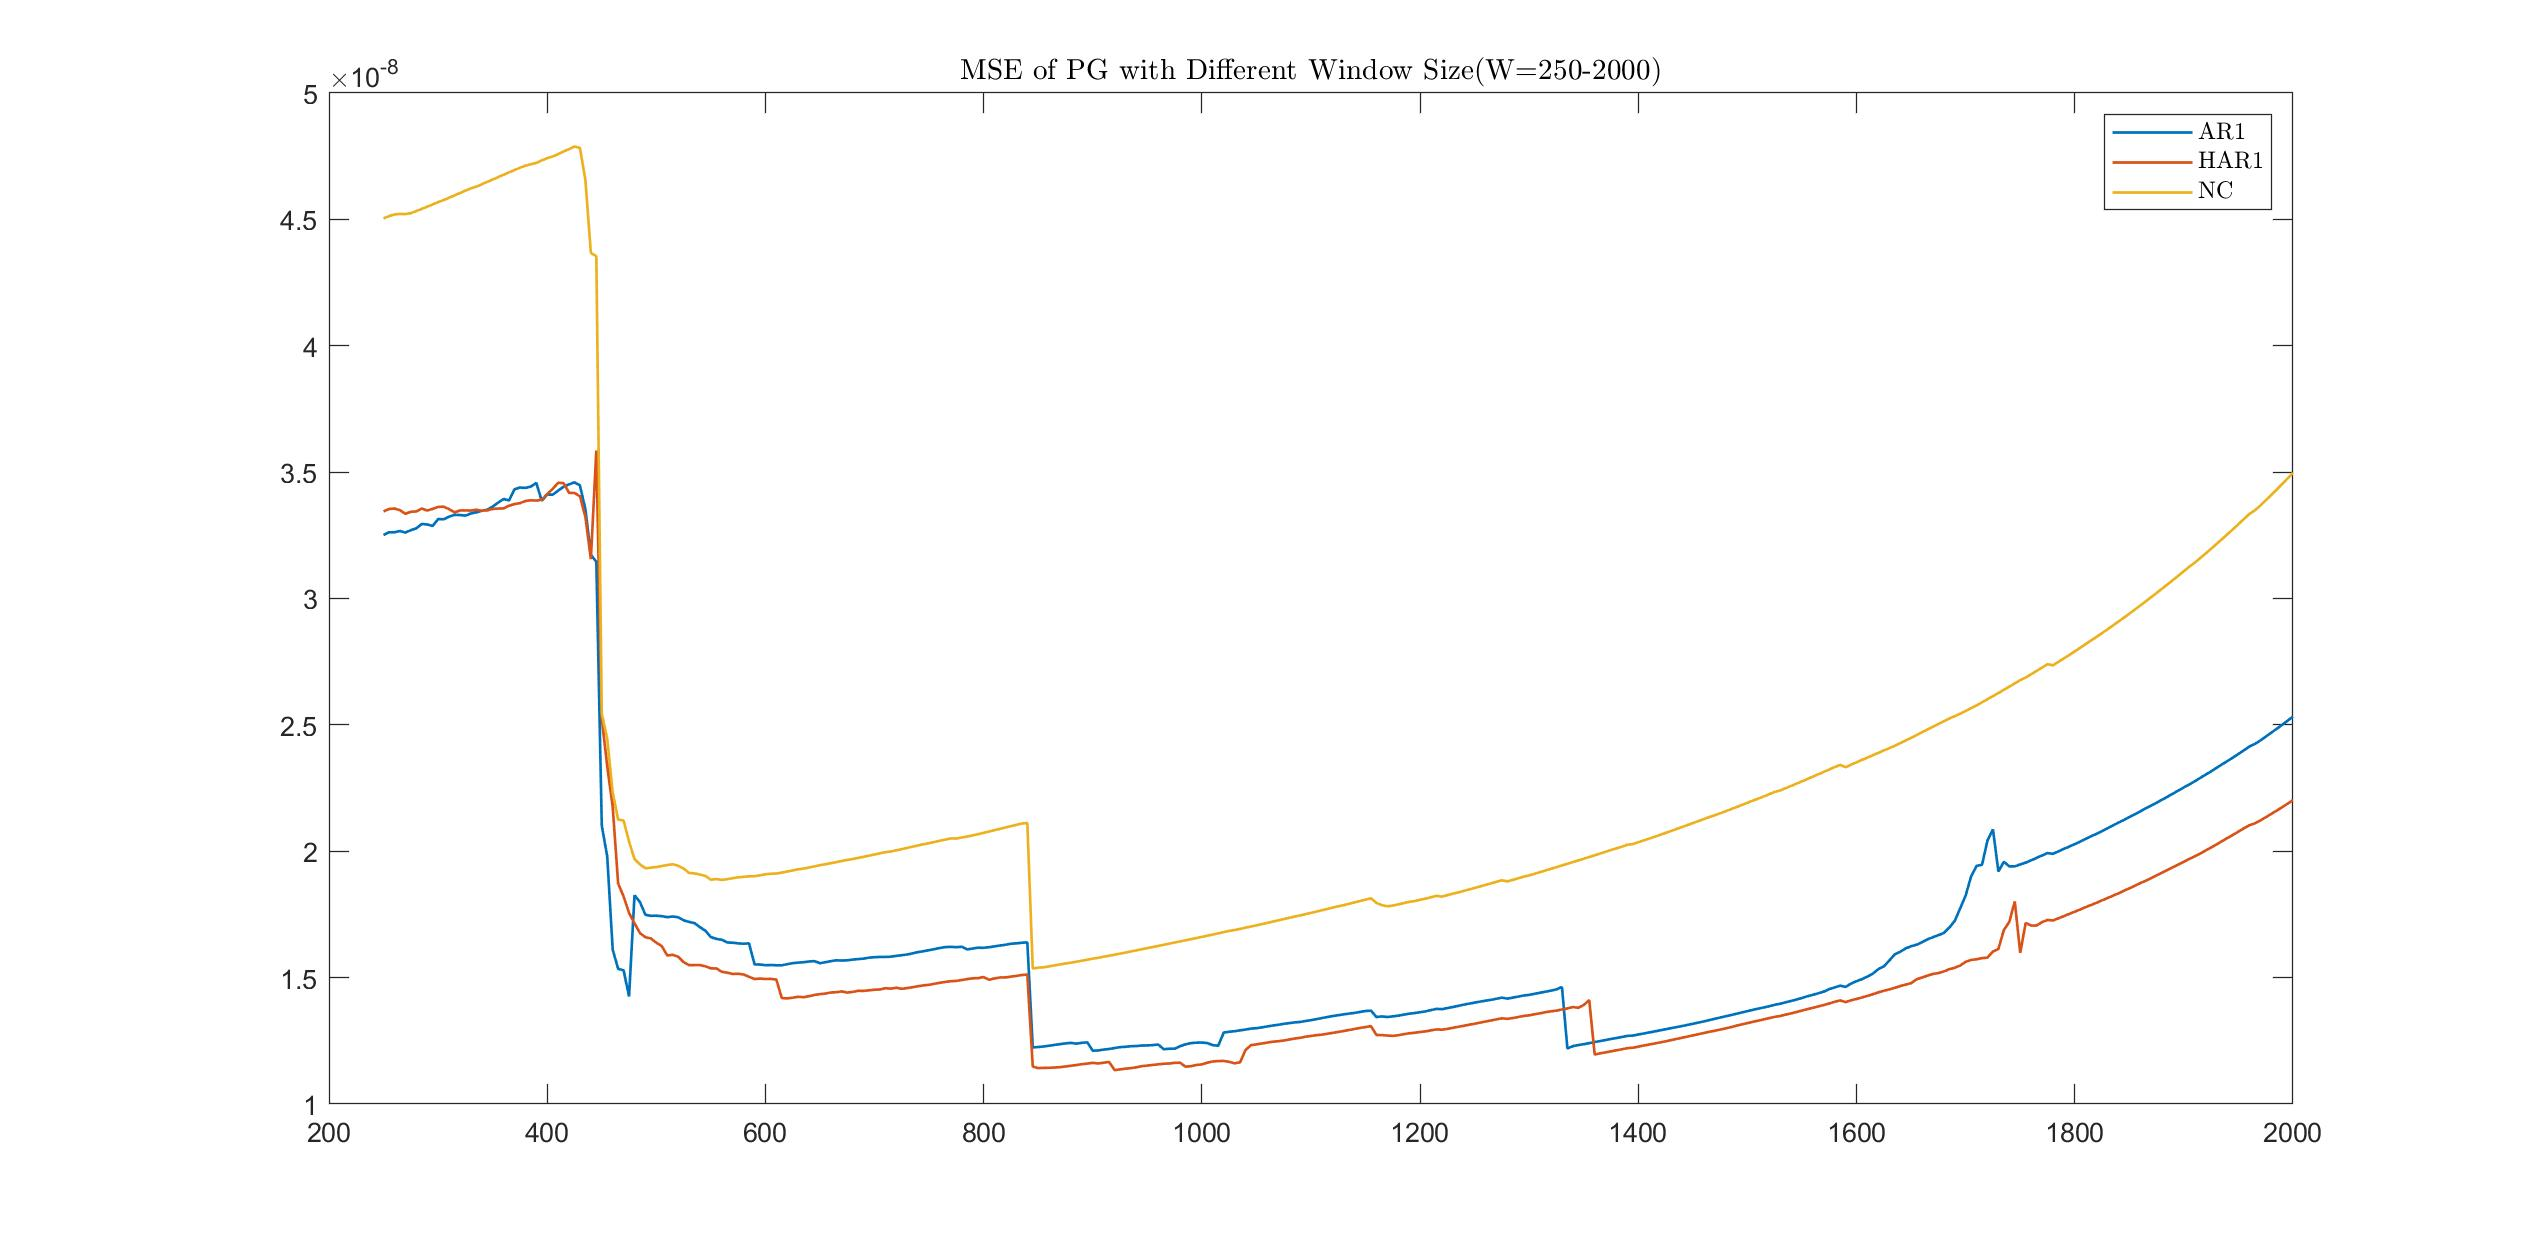
\includegraphics[width=12cm]{figures/1D_PG.jpg}
			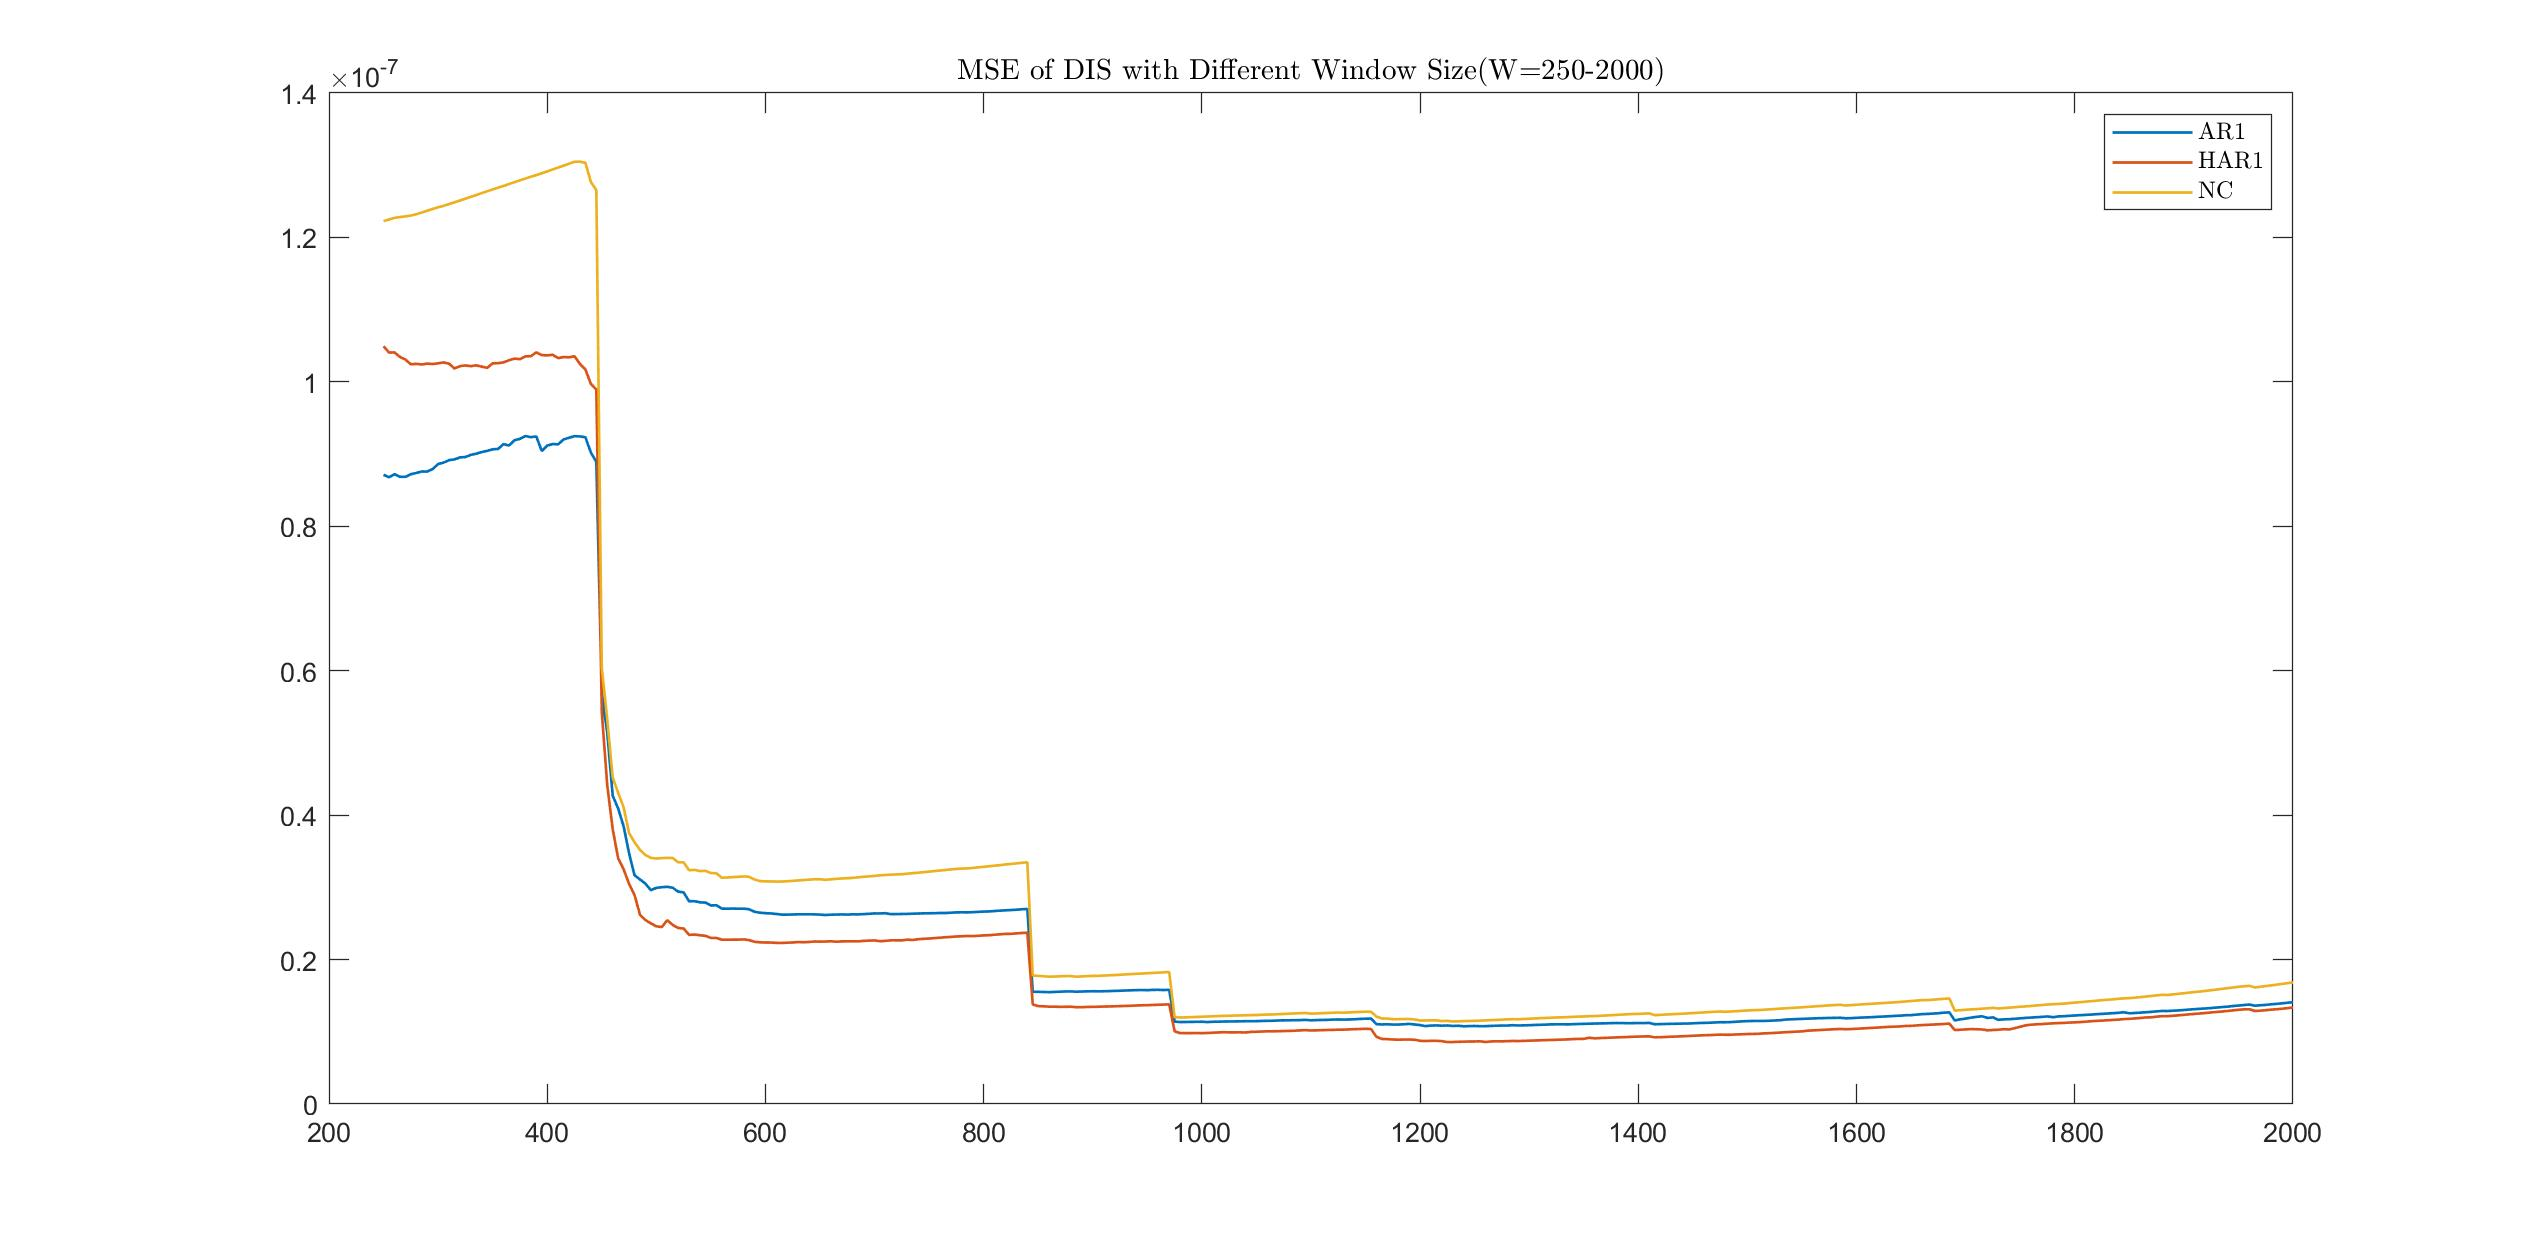
\includegraphics[width=12cm]{figures/1D_DIS.jpg}
		\end{minipage}
	}
	\centering
	\caption{MSE with Different Window Size}
\end{figure}

From the figure we can see, the MSE of forecast for these three models show a decrease jump at around J=500 and reach the lowest value at around J=1000. After reaching the lowest point, the MSE of PG starts increase, however, the MSE of DIS is persistent for increasing J.\\



The \textbf{MATLAB} code:

Function of Local Variance

Script of Q1
\lstinputlisting{scripts/ex6_Q1_PG.m}

\end{enumerate}
 

\newpage

%---------------------------------------------

\section*{Exercise 2-Errors in Variables (EIV)}
  \begin{enumerate}[label=\textbf{(\Alph*)}]
%---A---
\item The \textbf{MATLAB} code:
\lstinputlisting{functions/simulation.m}

In this function, $var1$ is the variance of $X$; $var2$ is the variance of error term $u$; $var3$ is the variance of $noise$. If $var3=0$, then the noise in $X$ is zero. 

%---B---
\item Here is the summary table of beta.
\begin{table}[ht]
	\footnotesize
	\caption{Summary Table of Parameter}
	\centering % used for centering table
	\begin{tabular}{lcc} % centered columns (4 columns)
		
		\hline %inserts double horizontal lines
		\hline % inserts single horizontal line
	Parameter&$\beta_0$&$\beta_1$\\ \hline
	Value&0.0376&1.0040\\
		
		\hline %inserts single line
		
	\end{tabular}
\end{table} 

%---C---
\item
Here are the histogram figures of $\beta_0$ and $\beta_1$.
 \begin{figure}[H]
	\subfigure{
		\begin{minipage}[l]{1\linewidth}
			\centering
			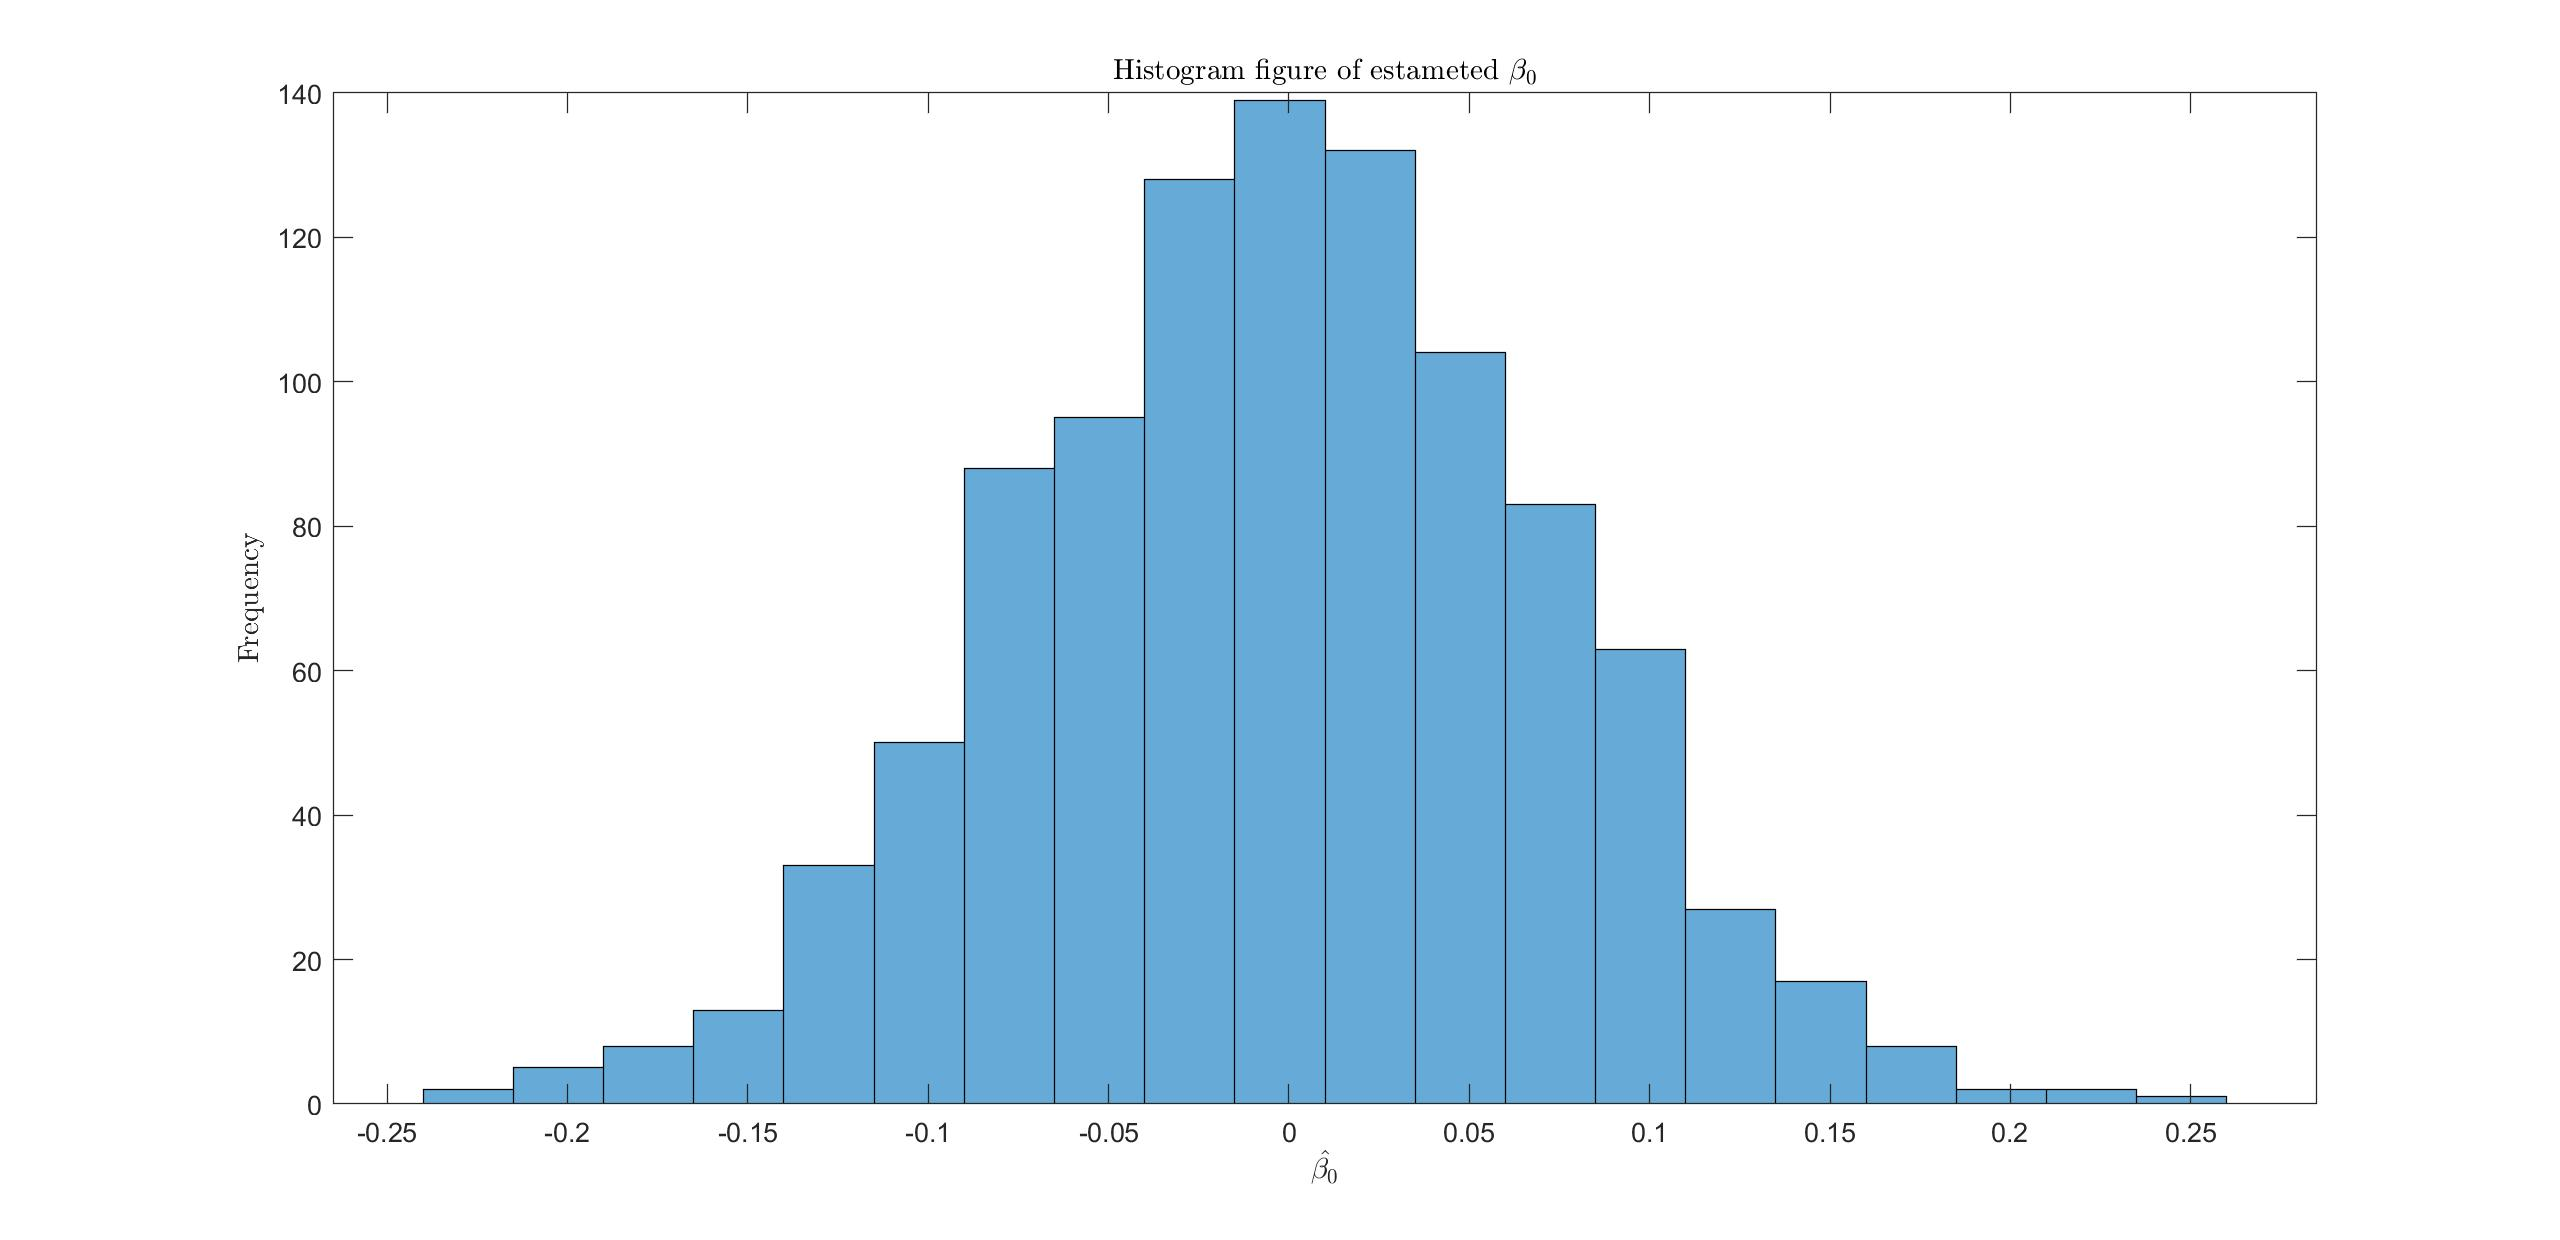
\includegraphics[width=3in]{figures/2C0.jpg}
			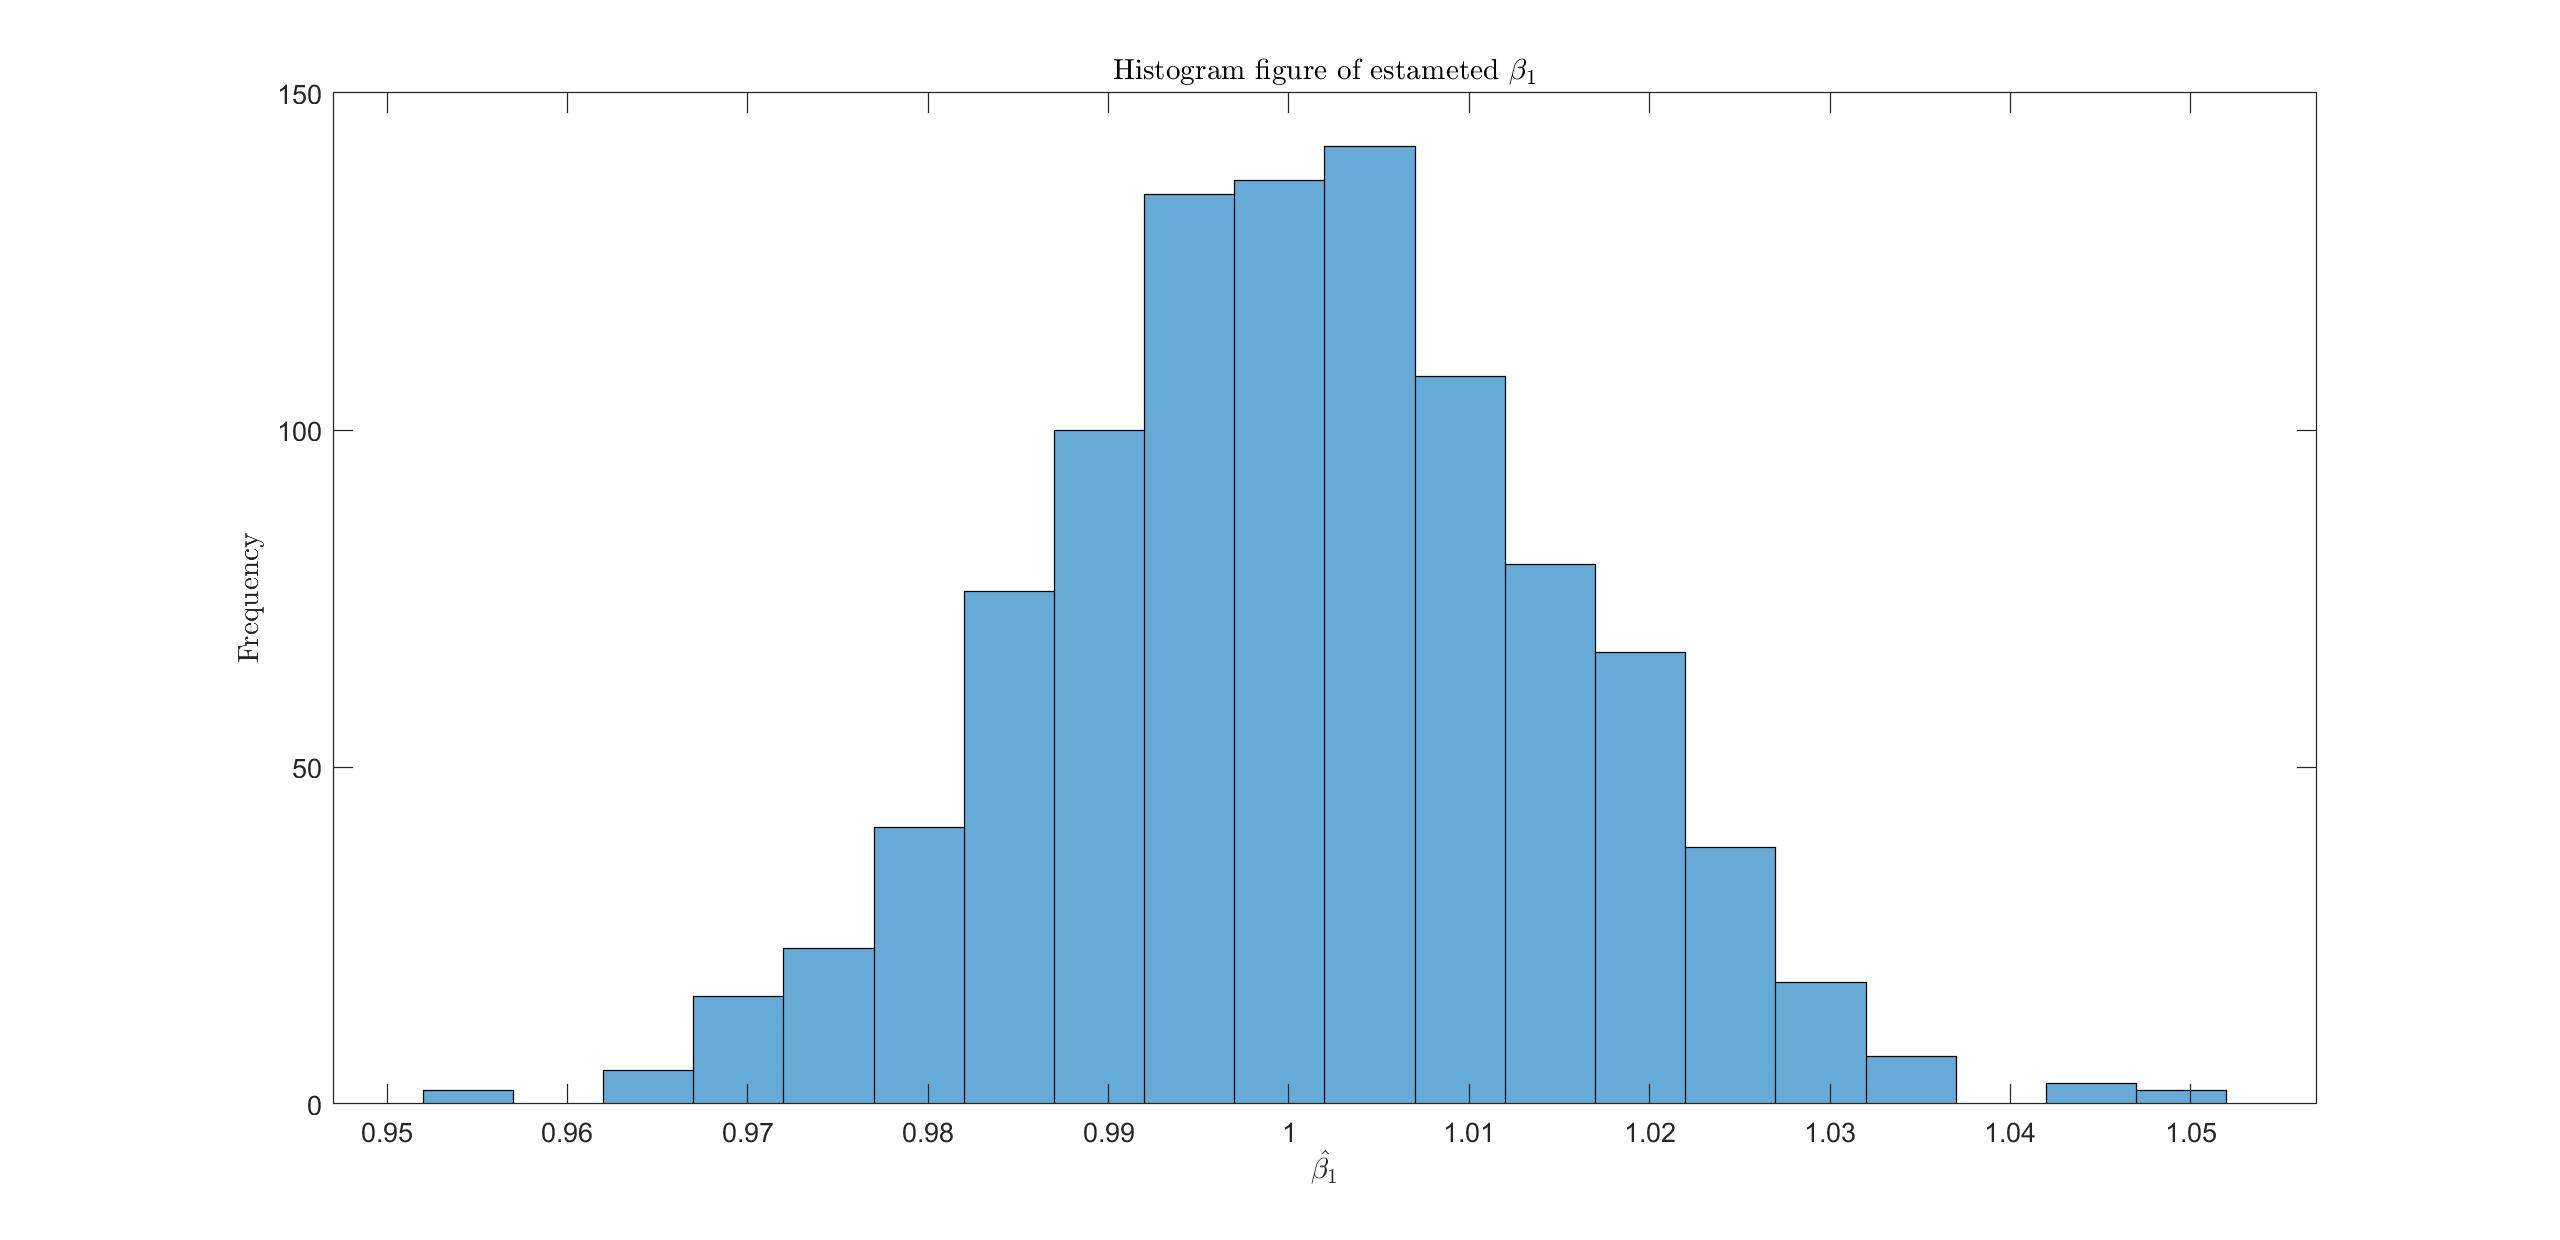
\includegraphics[width=3in]{figures/2C1.jpg}
		\end{minipage}
	}
	\centering
	\caption{ Histogram of $\beta_0$ and $\beta_1$}
\end{figure}

From the histogram figure of $\beta_0$ and $\beta_1$, we can see the shape of distribution of $\beta_0$ and $\beta_1$ is very similar to normal distribution. 

Specifically, the mean of $\beta_0$ showed in the plot is zero and the mean of $\beta_1$ is 1. The result satisfies our expectation.               

%---D---
\item
Here are the figures of estimated probability density function of $\beta_0$ and $\beta_1$.
\begin{figure}[H]
	\subfigure{
		\begin{minipage}[l]{1\linewidth}
			\centering
			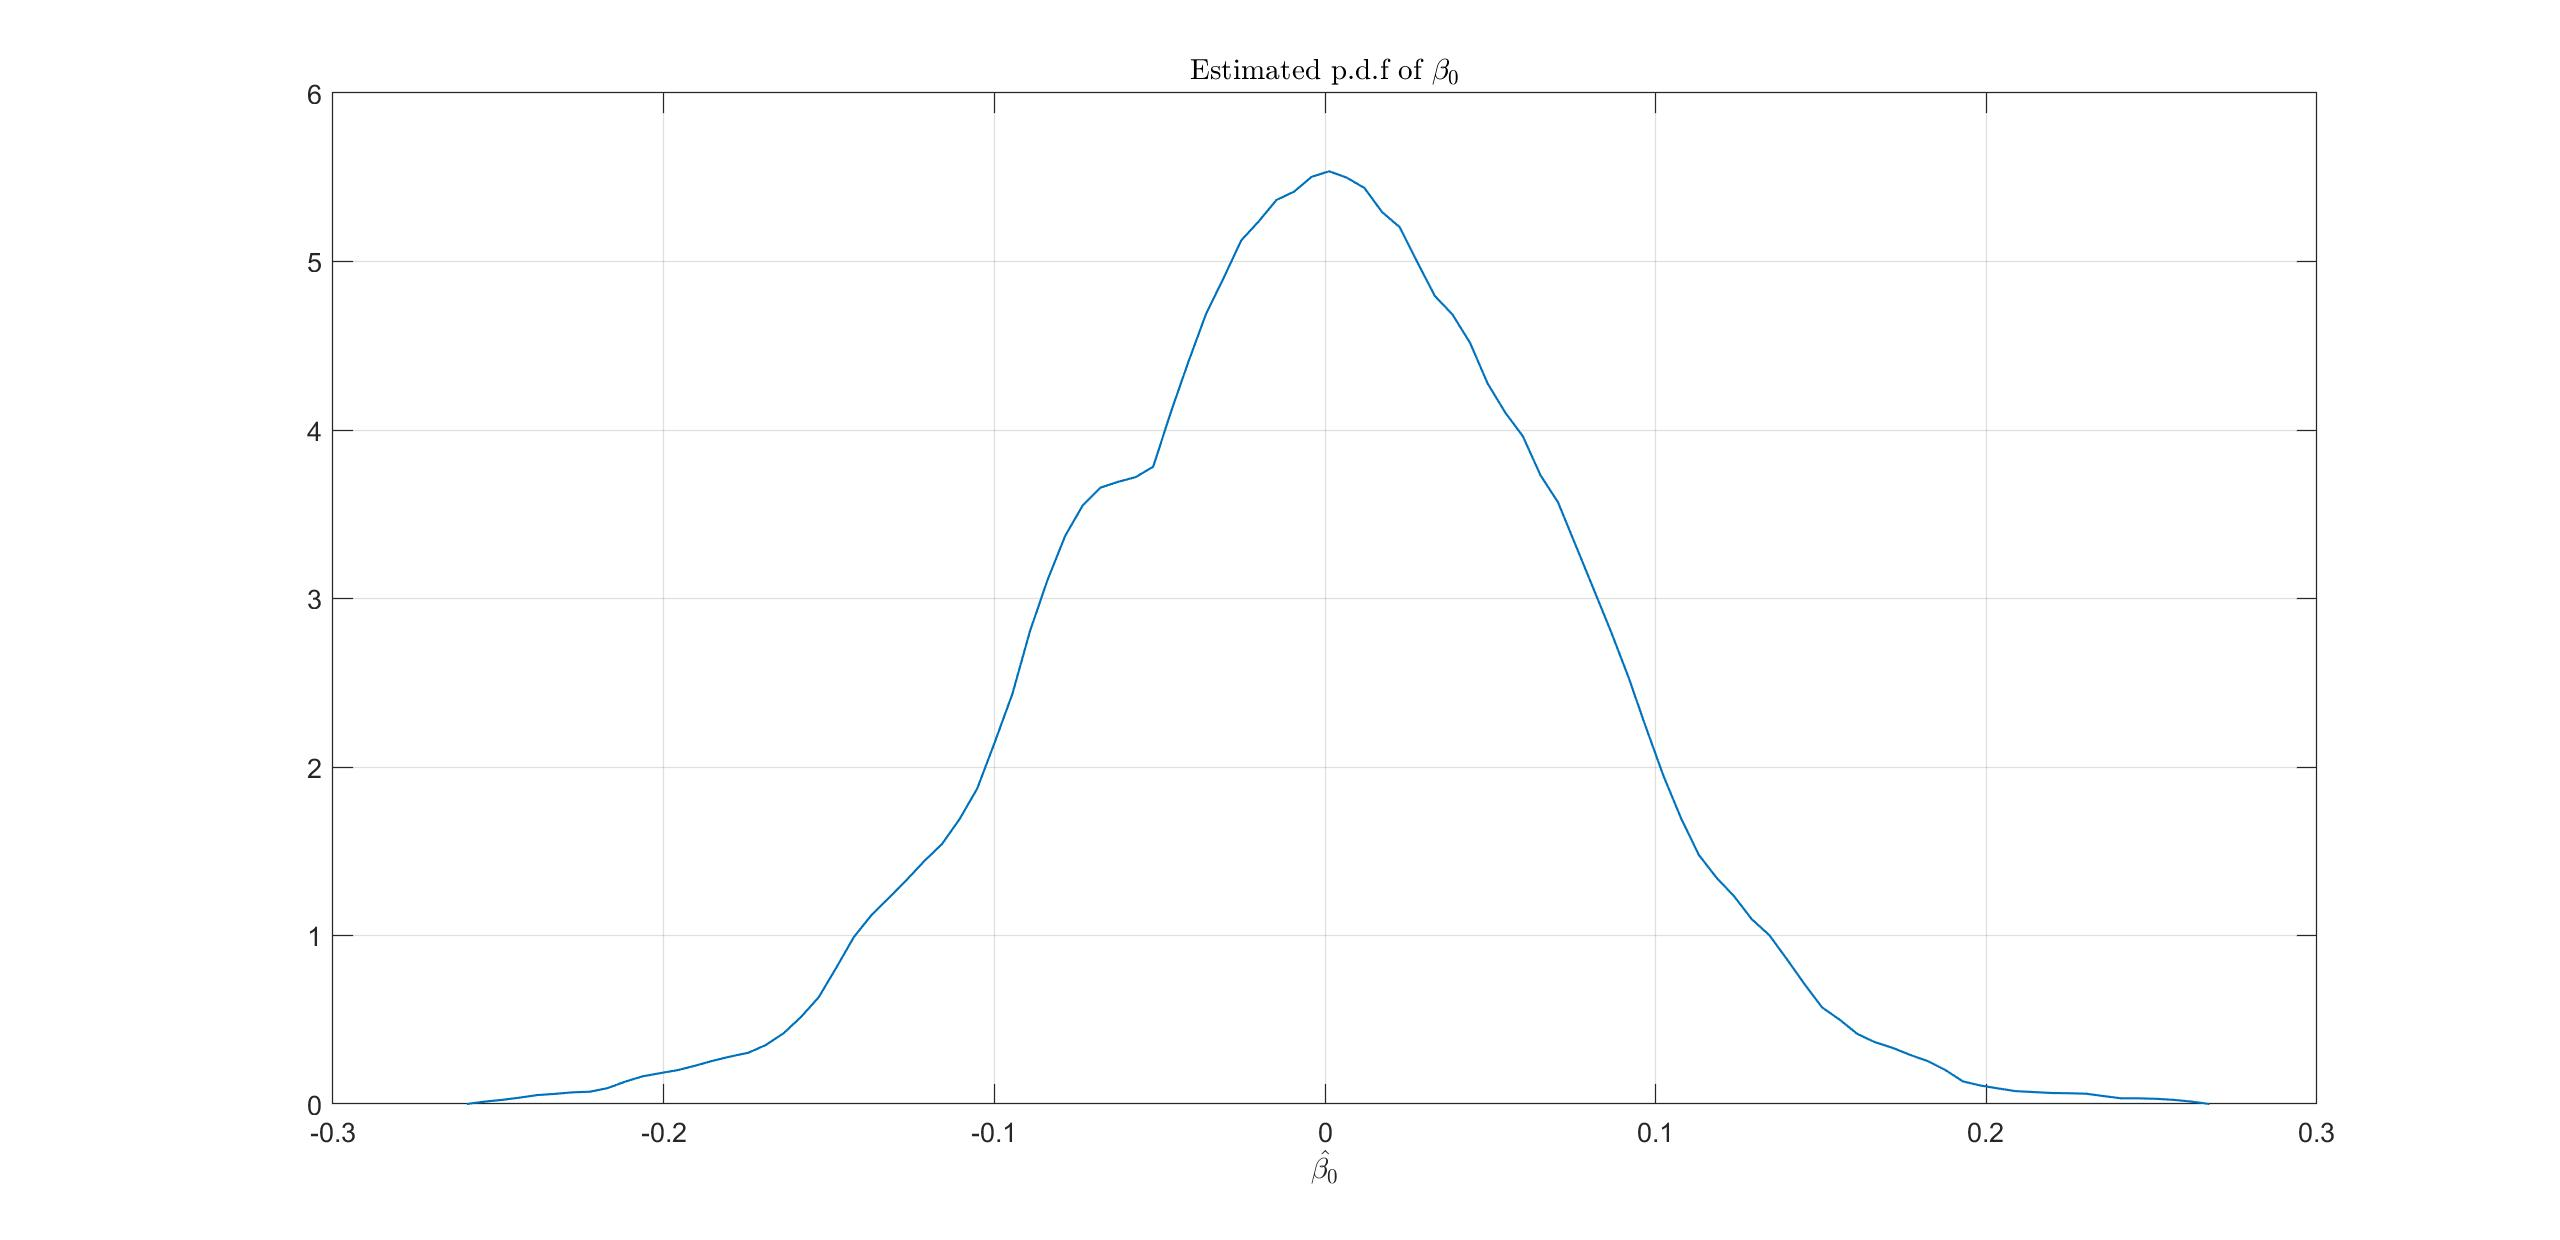
\includegraphics[width=3in]{figures/2D0.jpg}
			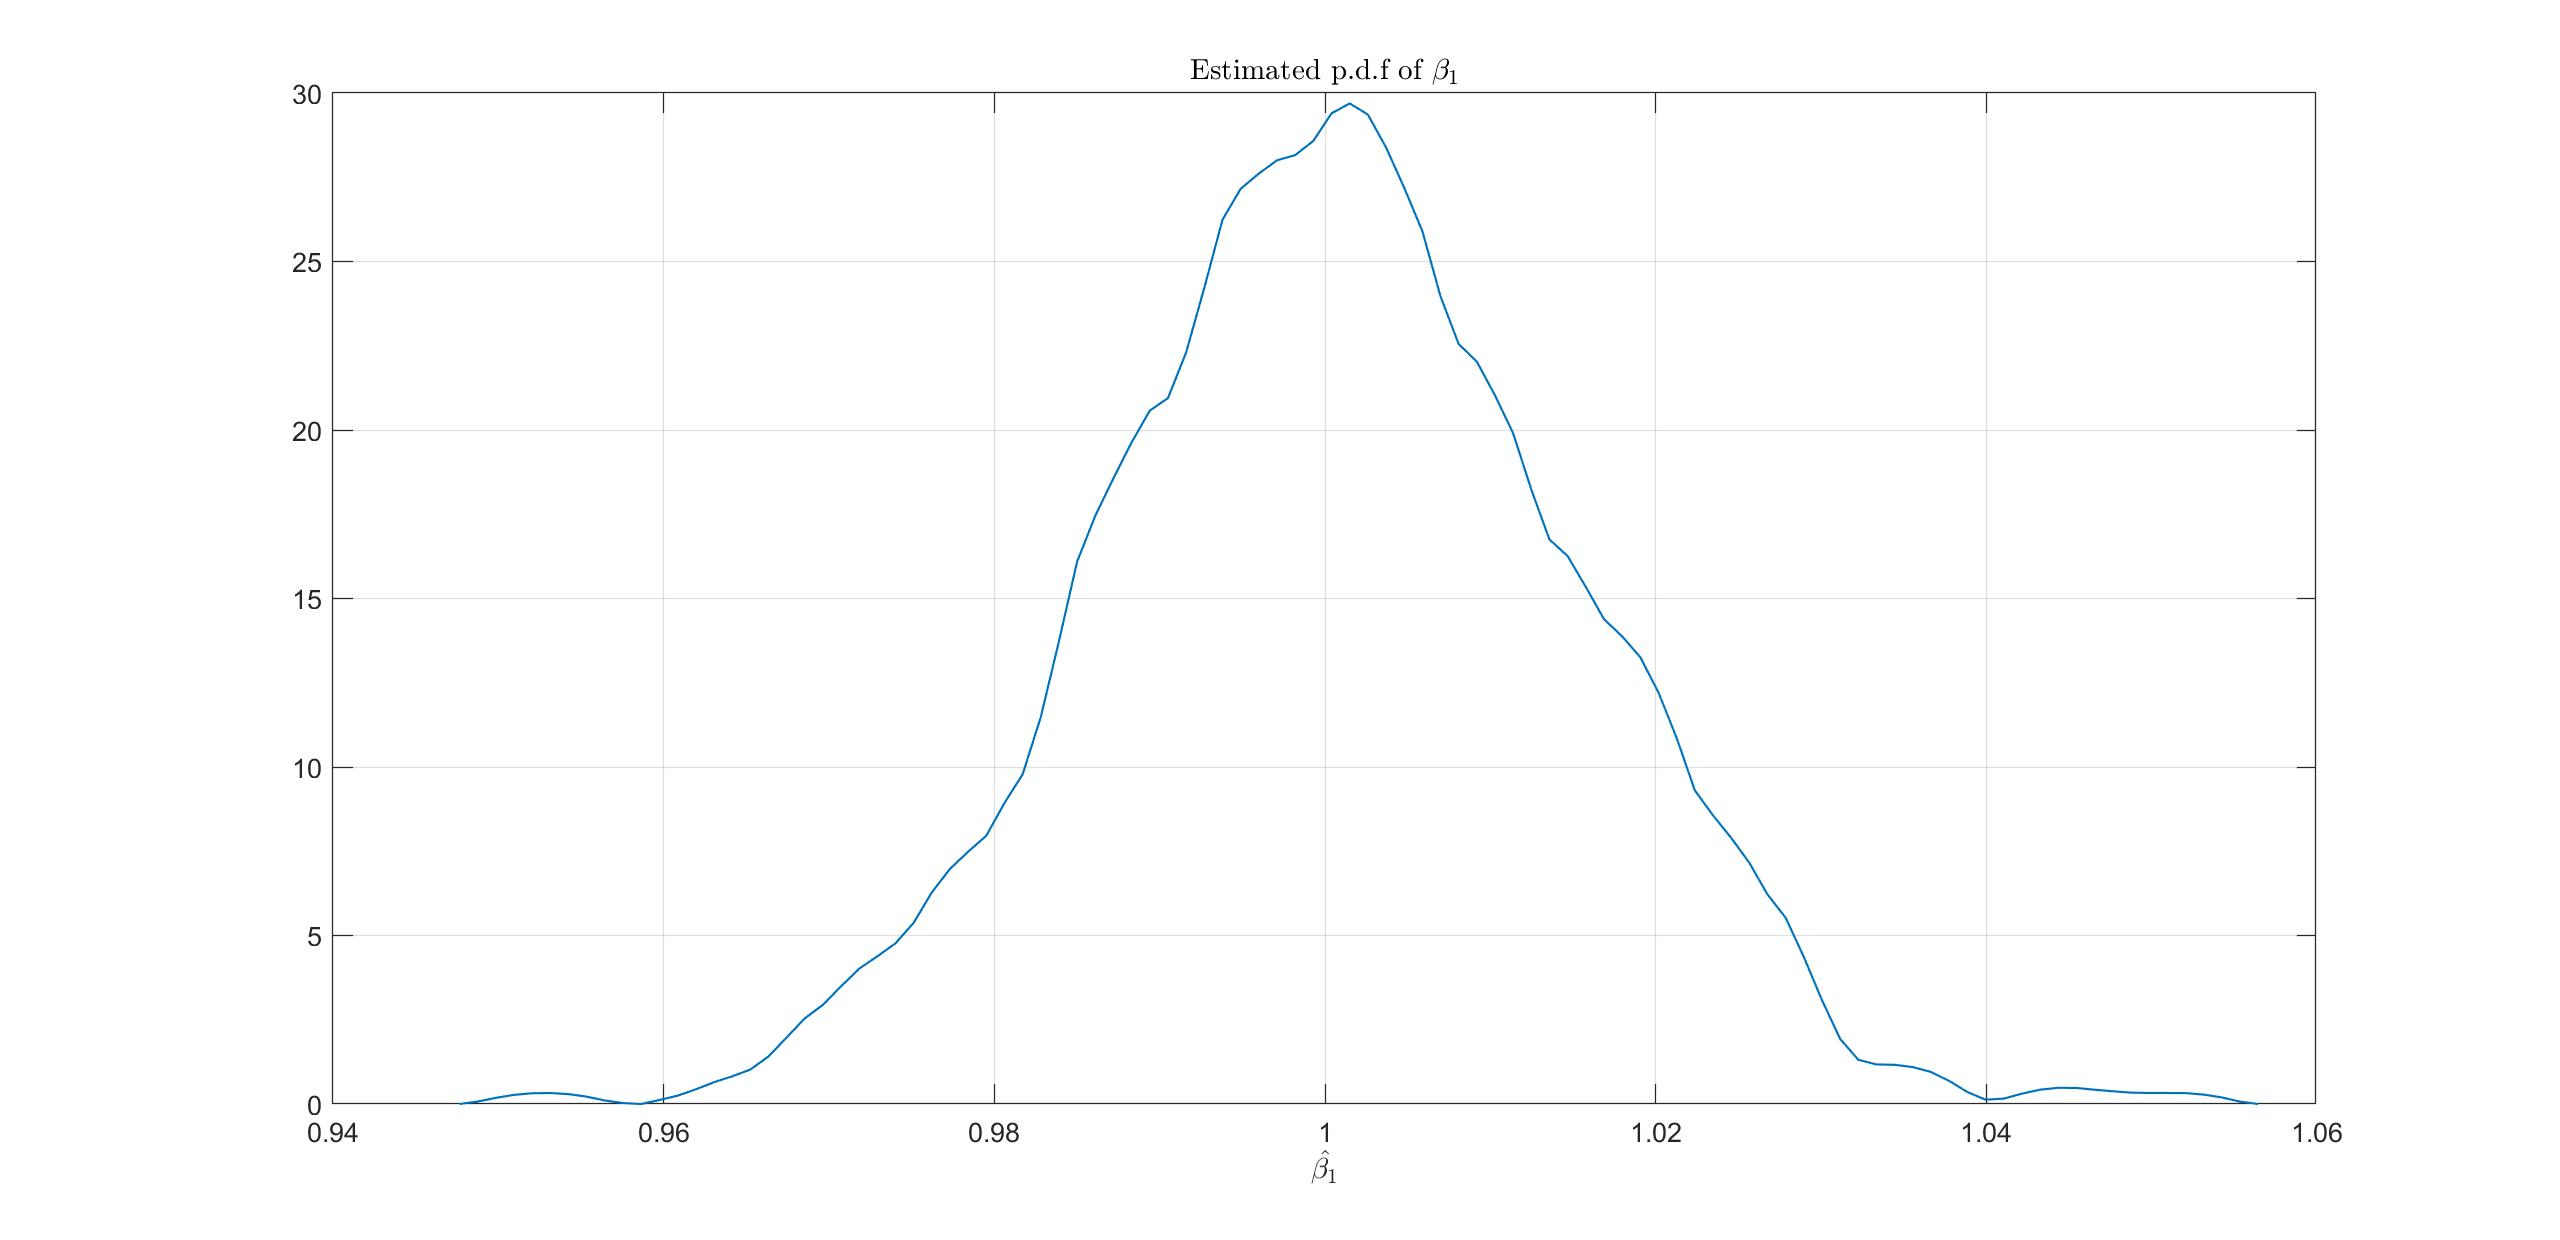
\includegraphics[width=3in]{figures/2D1.jpg}
		\end{minipage}
	}
	\centering
	\caption{ Estimated probability density function of $\beta_0$ and $\beta_1$}
\end{figure}

From the figures we can see the p.d.f. of $\beta_0$ and $\beta_1$ are very similar to normal distribution with mean equals to 0 and 1, respectively.  

Compare the distribution shape of $\beta_0$ and $\beta_1$ we can find: $\beta_0$'s distribution with a fatter tail and less peak, which indicates the variance of $\beta_0$ is larger than the variance of $\beta_1$. 



%---E---
\item 


For regression:
$$\tilde{Y_i}=\tilde{X_i}\beta+\tilde{u_i}$$
we can estimate $\beta$ by calculate:
$$\hat{\beta}^{ture}=\frac{Cov(\tilde{Y_i},\tilde{X_i})}{Var(\tilde{X_i})}=\frac{Cov(\tilde{X_i}\beta,\tilde{X_i})+Cov(\tilde{u_i},\tilde{X_i})}{Var(\tilde{X_i})}$$\\

If some noises are added into $\tilde{X_i}$, the regression with noise will be:
$$\tilde{Y_i}=\tilde{X_i^{*}}\beta^{*}+\tilde{u_i}$$
where $\tilde{X_i^{*}}=\tilde{X_i}+\eta_i$ is the noise version of $\tilde{X_i}$.
we can estimate $\beta^{*}$ by calculate:
$$\hat{\beta}^{*}=\frac{Cov(\tilde{Y_i},\tilde{X_i^{*}})}{Var(\tilde{X_i^{*}})}=\frac{Cov(\tilde{X_i}\beta,\tilde{X_i})+Cov(\tilde{u_i},\tilde{X_i})+Cov(\tilde{X_i}\beta,\eta_i)+Cov(\tilde{u_i},\eta_i)}{Var(\tilde{X_i})+Var(\eta)+Cov(\tilde{X_i},\eta_i)}$$

Assume noises $\eta_i$ are uncorrelated with $\tilde{X_i}$, we can simplify $\hat{\beta}^{*}$ as:
$$\hat{\beta}^{*}=\frac{Cov(\tilde{X_i}\beta,\tilde{X_i})+Cov(\tilde{u_i},\tilde{X_i})}{Var(\tilde{X_i})+Var(\eta)}$$

as the $Var(\eta)$ increases,  $\hat{\beta}^{*}$ will decrease and we will get a down-biased estimator of $\beta$. For the rest part, noises will be added to X to see how it affect the estimation of parameter $\beta$.\\
\newpage

We first change the variance of $noise$ from 0 to $0.30\sigma_x^2$.
\begin{enumerate}[label=(\roman*)]
%---EB---
\item Here is the summary table of estimate value of $\hat{\beta_0}^{*}$ and $\hat{\beta_1}^{*}$.
\begin{table}[ht]
	\footnotesize
	\caption{Summary Table of Parameter}
	\centering % used for centering table
	\begin{tabular}{lcc} % centered columns (4 columns)
		
		\hline %inserts double horizontal lines
		%heading
		\hline % inserts single horizontal line
		Parameter&$\hat{\beta_0}^{*}$ & $\hat{\beta_1}^{*}$\\
		Value&0.1643&0.9881\\
		
		\hline %inserts single line
		
	\end{tabular}
\end{table} 

%---EC---
\item Here are the histogram figures of $\hat{\beta_0}^{*}$ and $\hat{\beta_1}^{*}$.
\begin{figure}[H]
	\subfigure{
		\begin{minipage}[l]{1\linewidth}
			\centering
			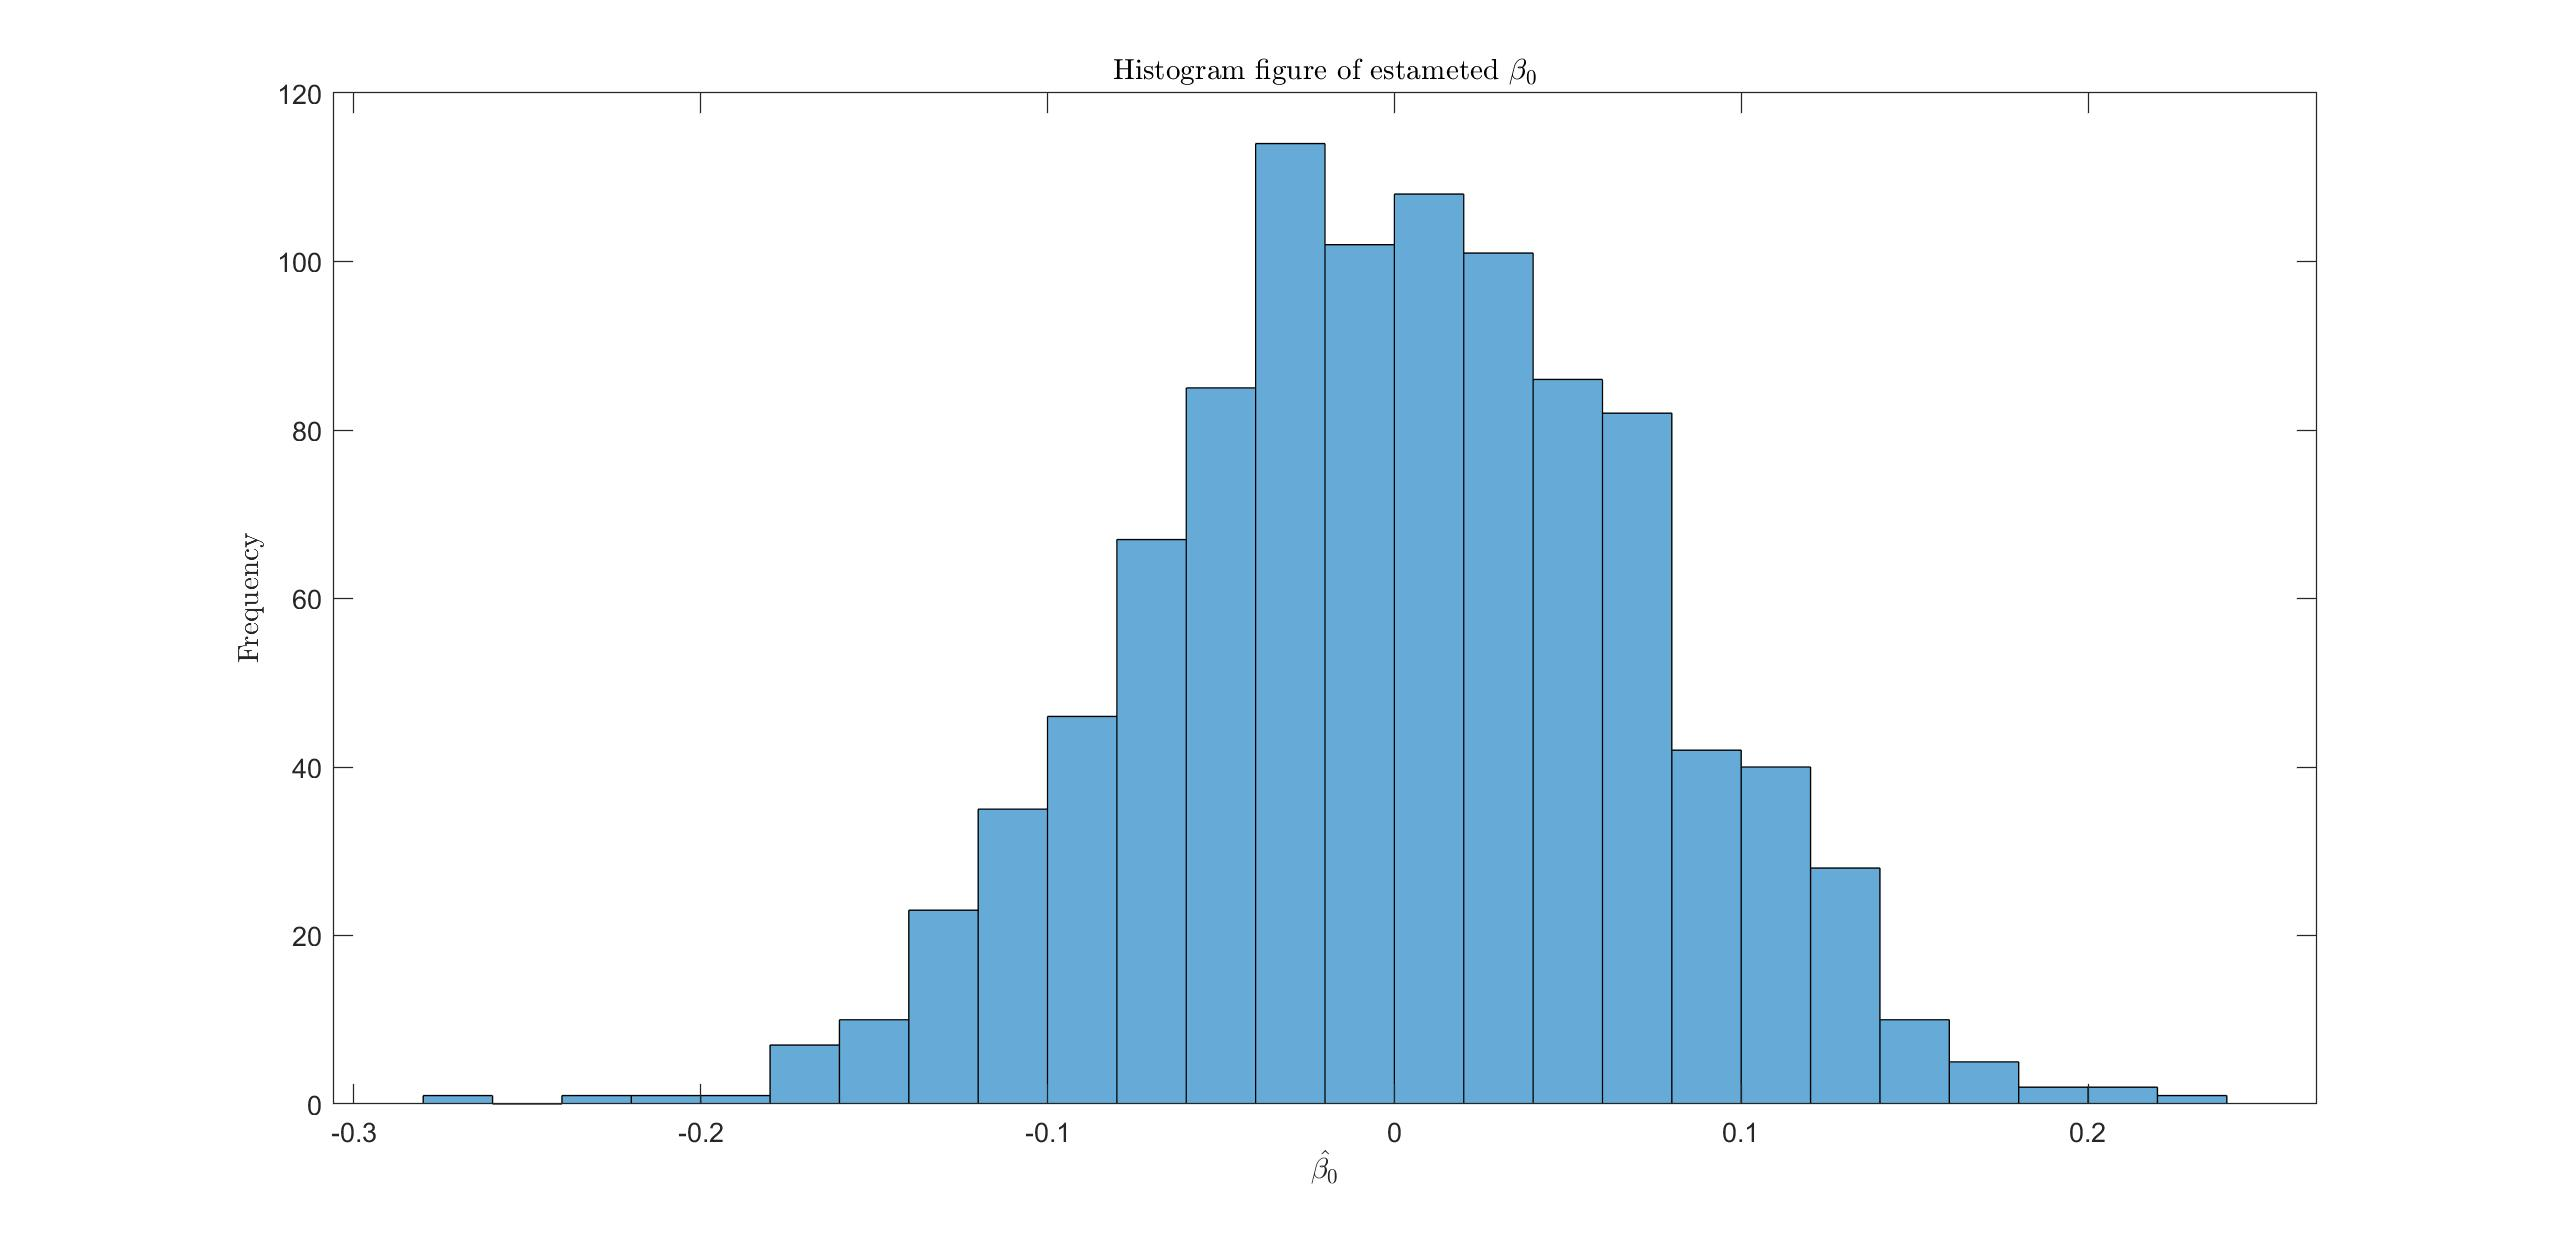
\includegraphics[width=3in]{figures/2Eh0.jpg}
			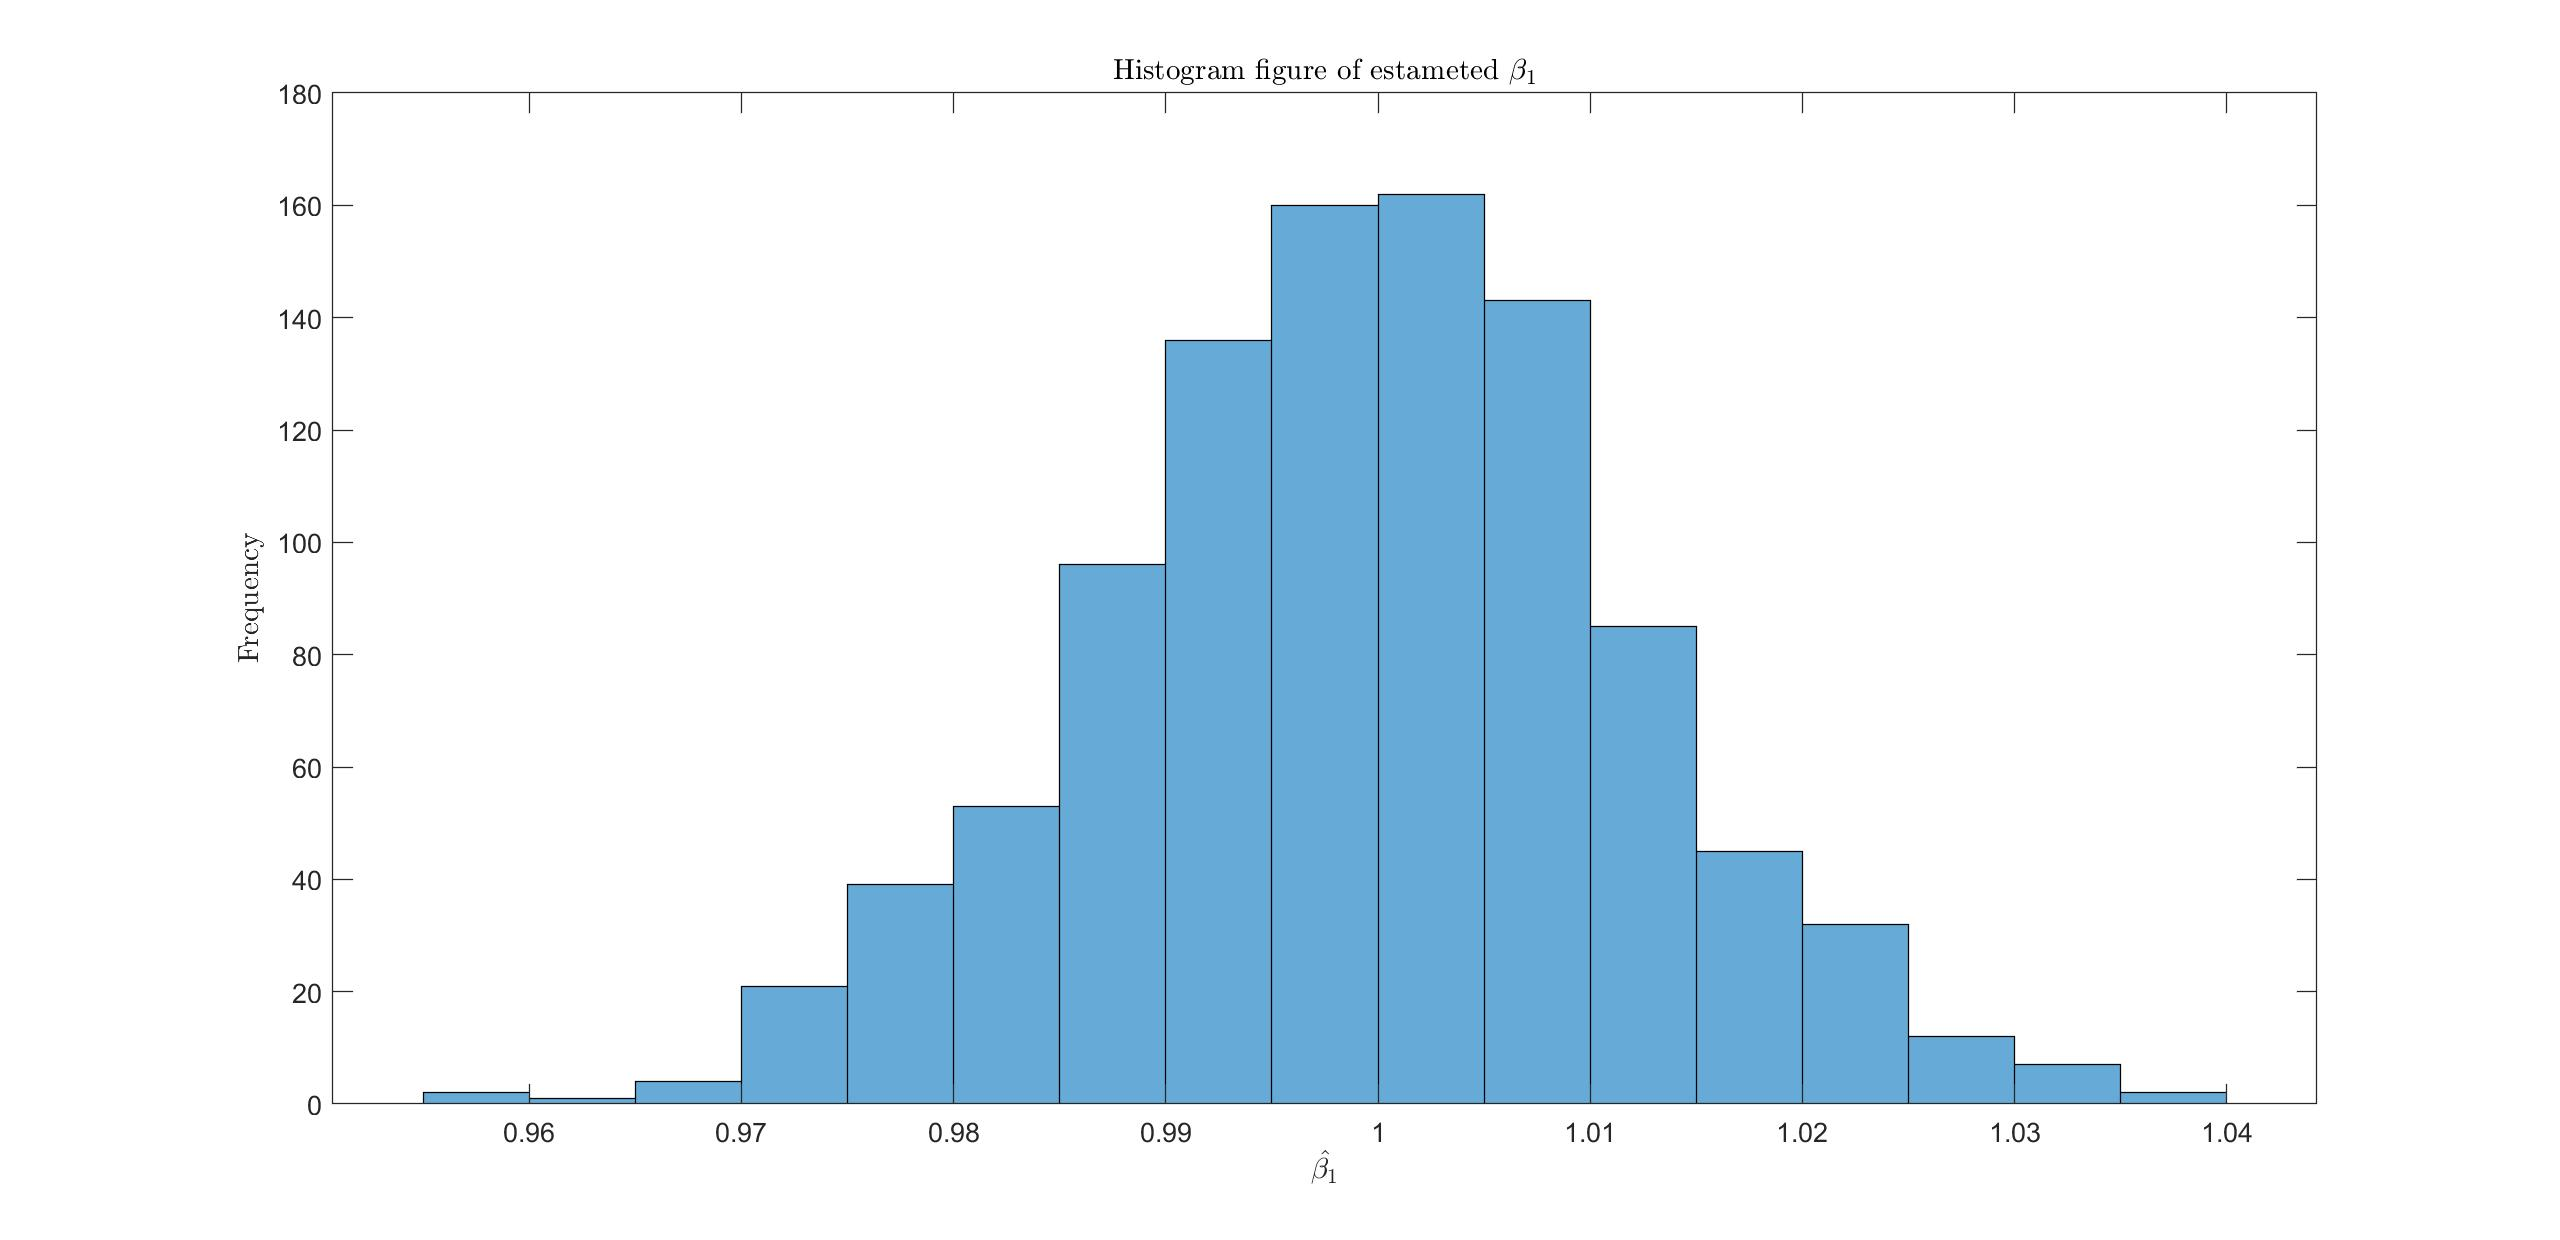
\includegraphics[width=3in]{figures/2Eh1.jpg}
		\end{minipage}
	}
	\centering
	\caption{ Histogram of $\hat{\beta_0}^{*}$ and $\hat{\beta_1}^{*}$}
\end{figure}

%---ED---

\item Here are the figures of estimated probability density function of $\hat{\beta_0}^{*}$ and $\hat{\beta_1}^{*}$.
\begin{figure}[H]
	\subfigure{
		\begin{minipage}[l]{1\linewidth}
			\centering
			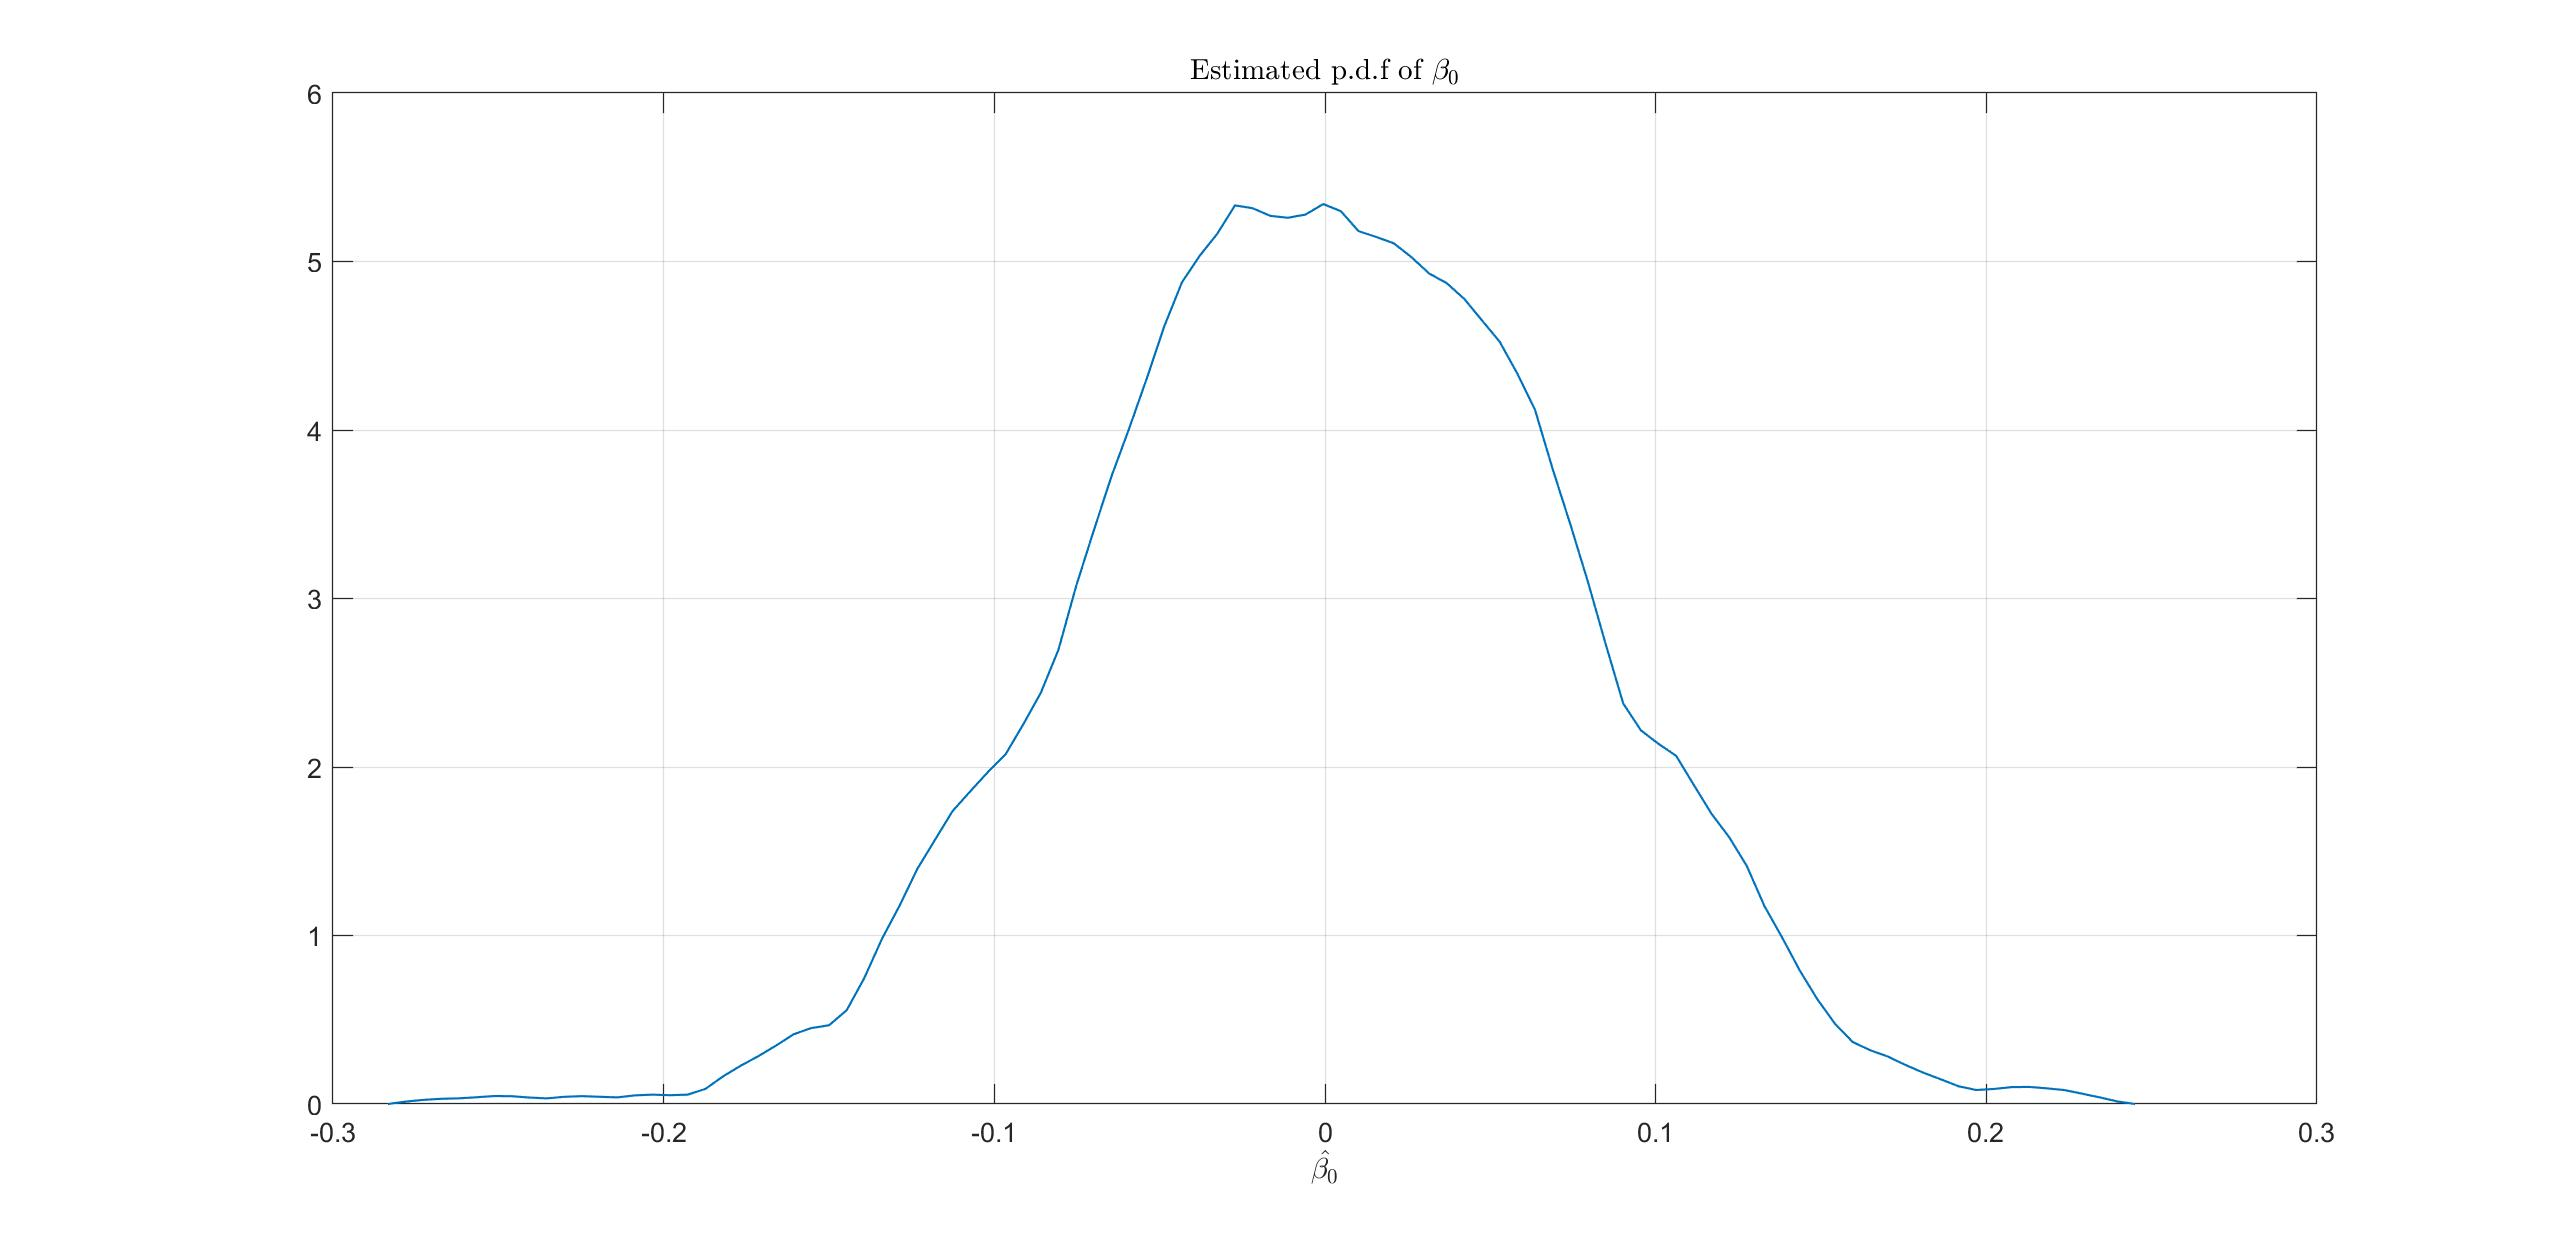
\includegraphics[width=3in]{figures/2Ef0.jpg}
			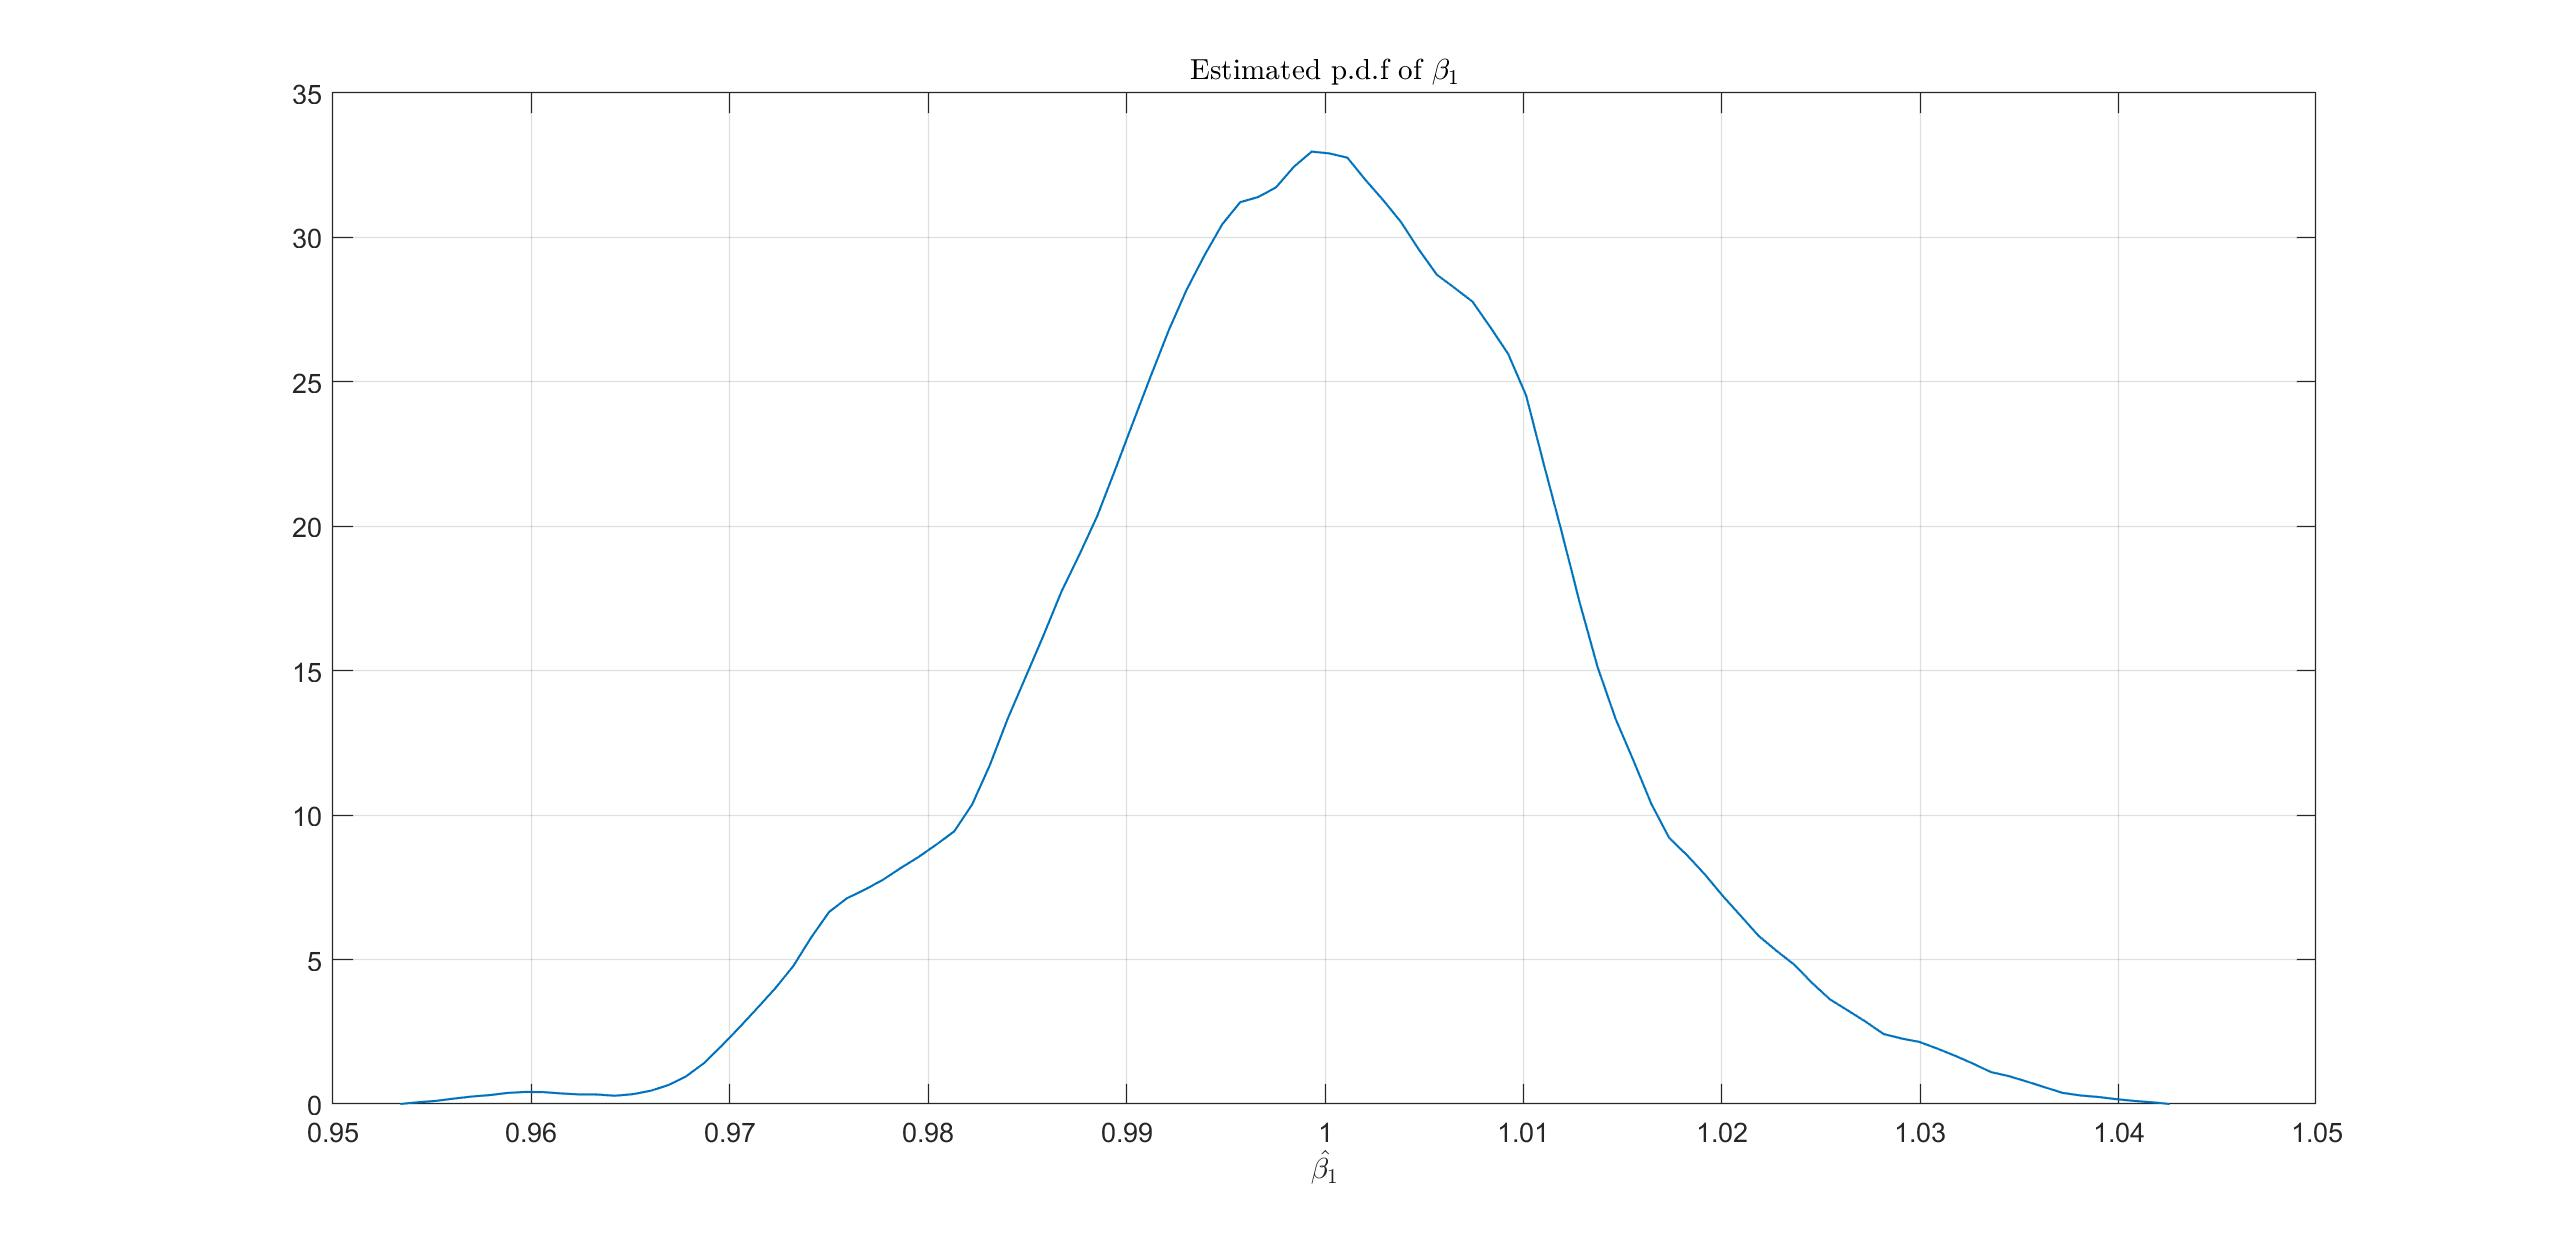
\includegraphics[width=3in]{figures/2Ef1.jpg}
		\end{minipage}
	}
	\centering
	\caption{Estimated probability density function of $\hat{\beta_0}^{*}$ and $\hat{\beta_1}^{*}$}
\end{figure}
\end{enumerate}
From the figures we can see the shape of distribution of $\hat{\beta_0}^{*}$ and $\hat{\beta_1}^{*}$ are still similar to normal distribution, but they show a trend of left skew and the mean of $\hat{\beta_0}^{*}$ and $\hat{\beta_1}^{*}$ in the estimated distribution are a little smaller than 0 and 1, respectively.\\
\newpage


%----2F----
\item 
We then change the variance of $\eta_i$ to $0.50\sigma_x^2$.
\begin{enumerate}[label=(\roman*)]
	%---2FB---
	\item Here is the summary table of estimate value of $\hat{\beta_0}^{*}$ and $\hat{\beta_1}^{*}$.
	\begin{table}[ht]
		\footnotesize
		\caption{Summary Table of Parameter}
		\centering % used for centering table
		\begin{tabular}{lcc} % centered columns (4 columns)
			
			\hline%inserts double horizontal lines
		 % inserts table	%heading
			\hline % inserts single horizontal line
			Parameter&$\hat{\beta_0}^{*}$ & $\hat{\beta_1}^{*}$\\ \hline
			Value&0.0338&0.9835\\
			\hline %inserts single line
			
		\end{tabular}
	\end{table} 
	
	%---2FC---
\item	Here are the histogram figures of $\hat{\beta_0}^{*}$ and $\hat{\beta_1}^{*}$.
	\begin{figure}[H]
		\subfigure{
			\begin{minipage}[l]{1\linewidth}
				\centering
				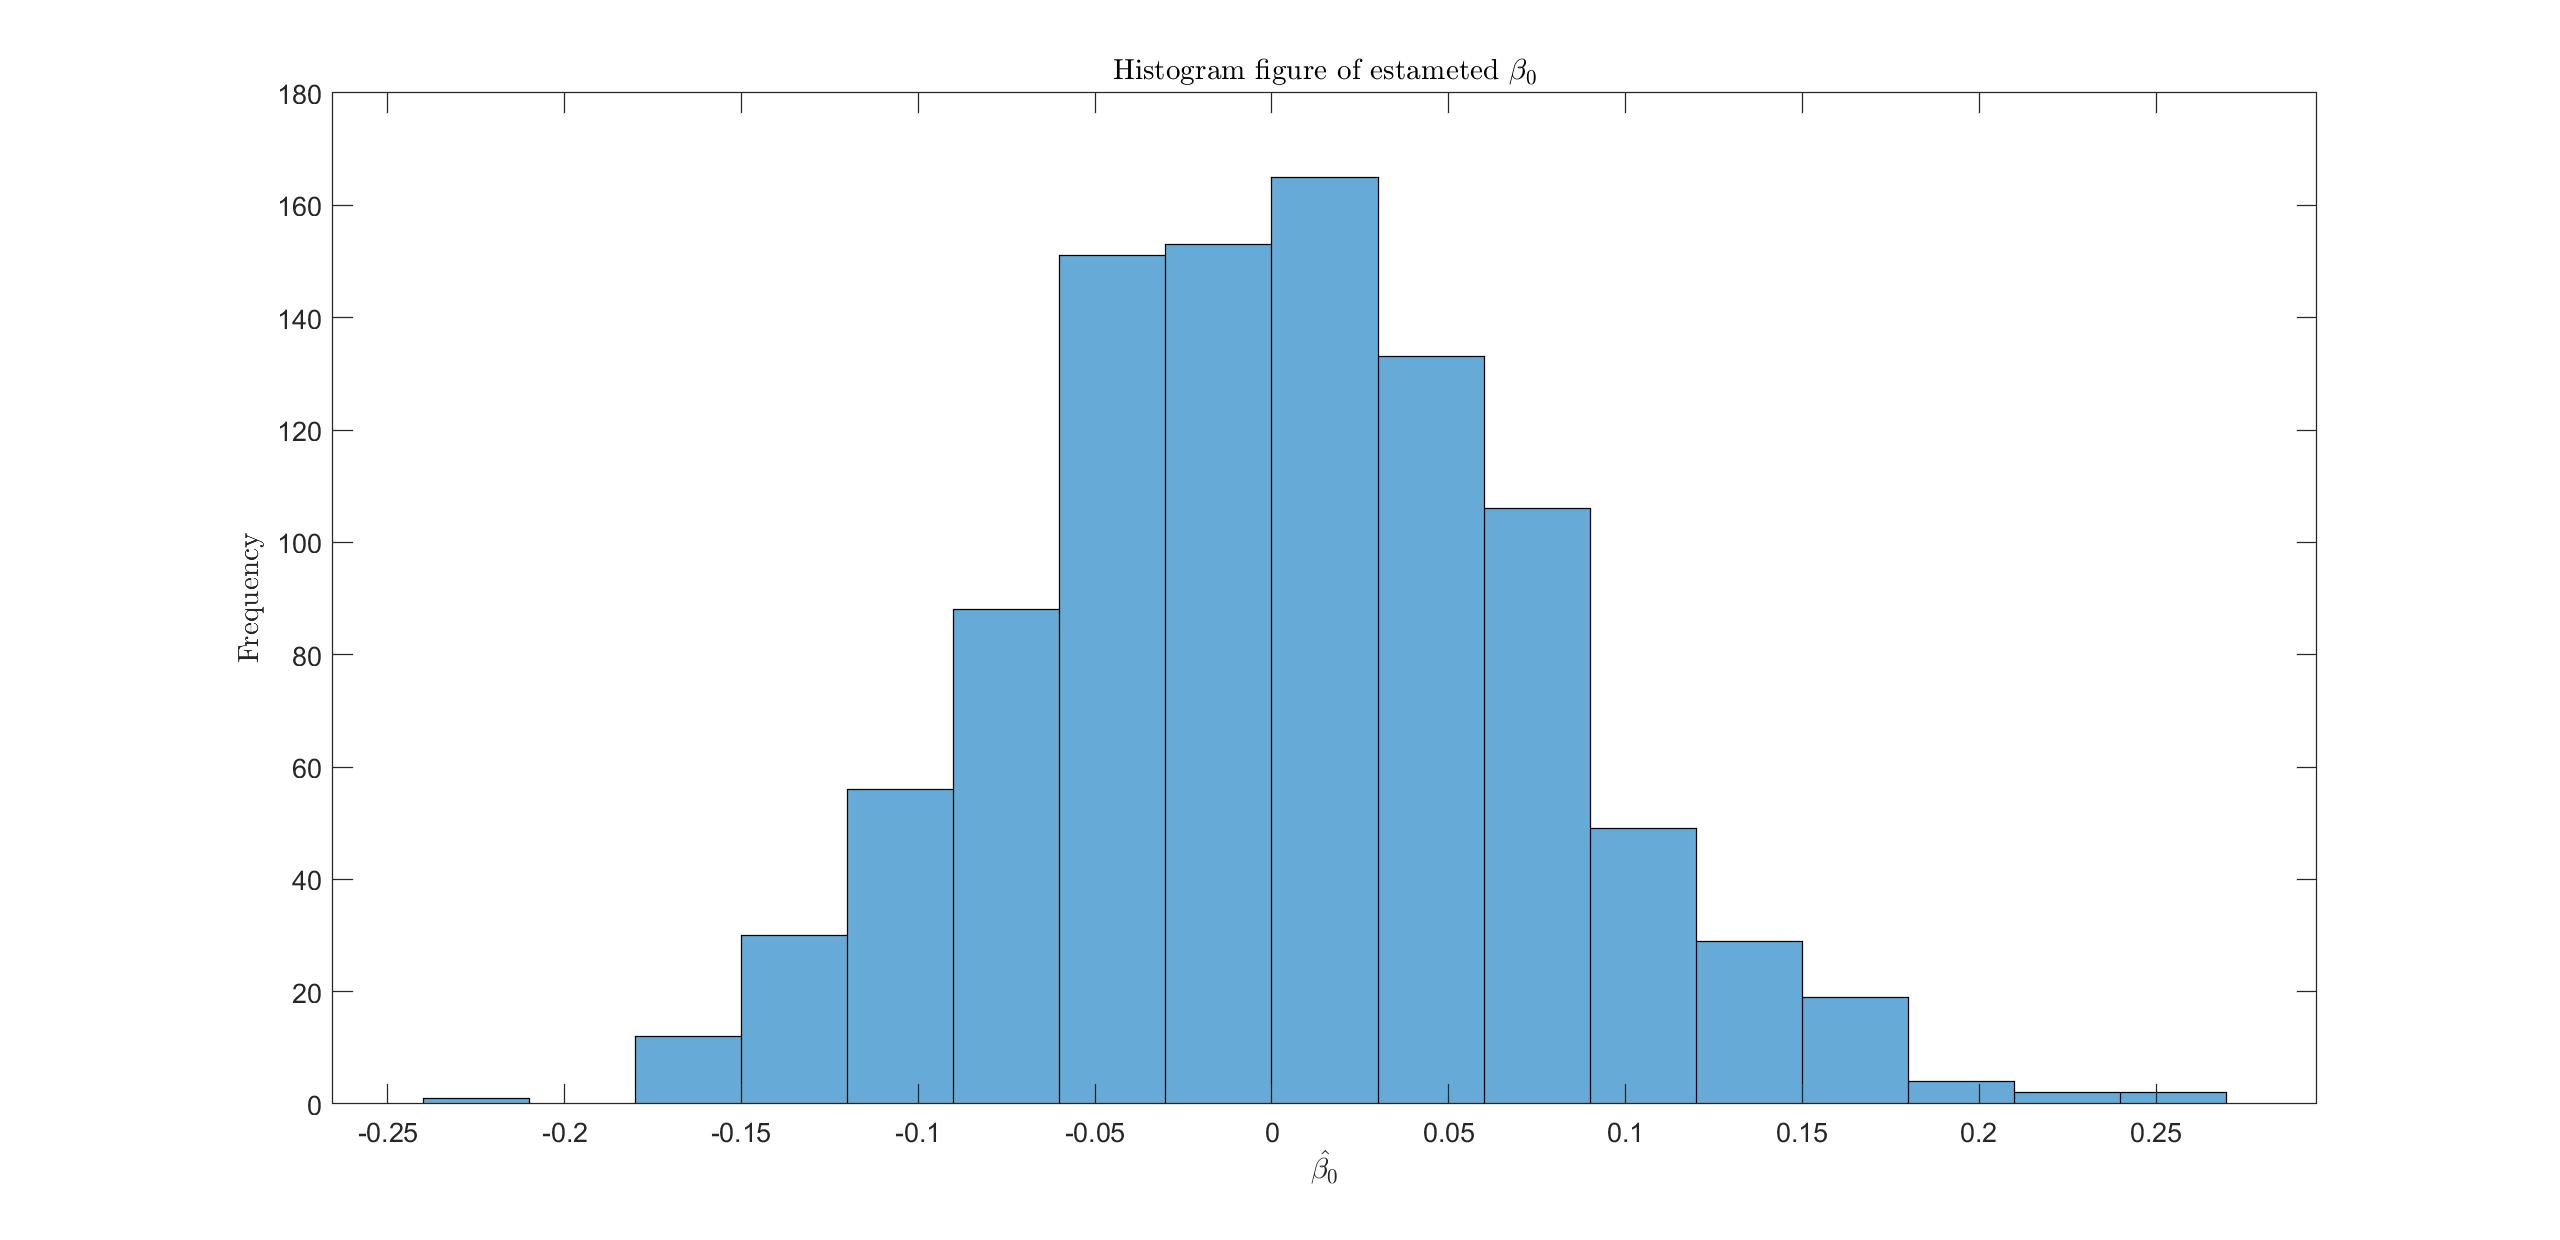
\includegraphics[width=3in]{figures/2Fh0.jpg}
				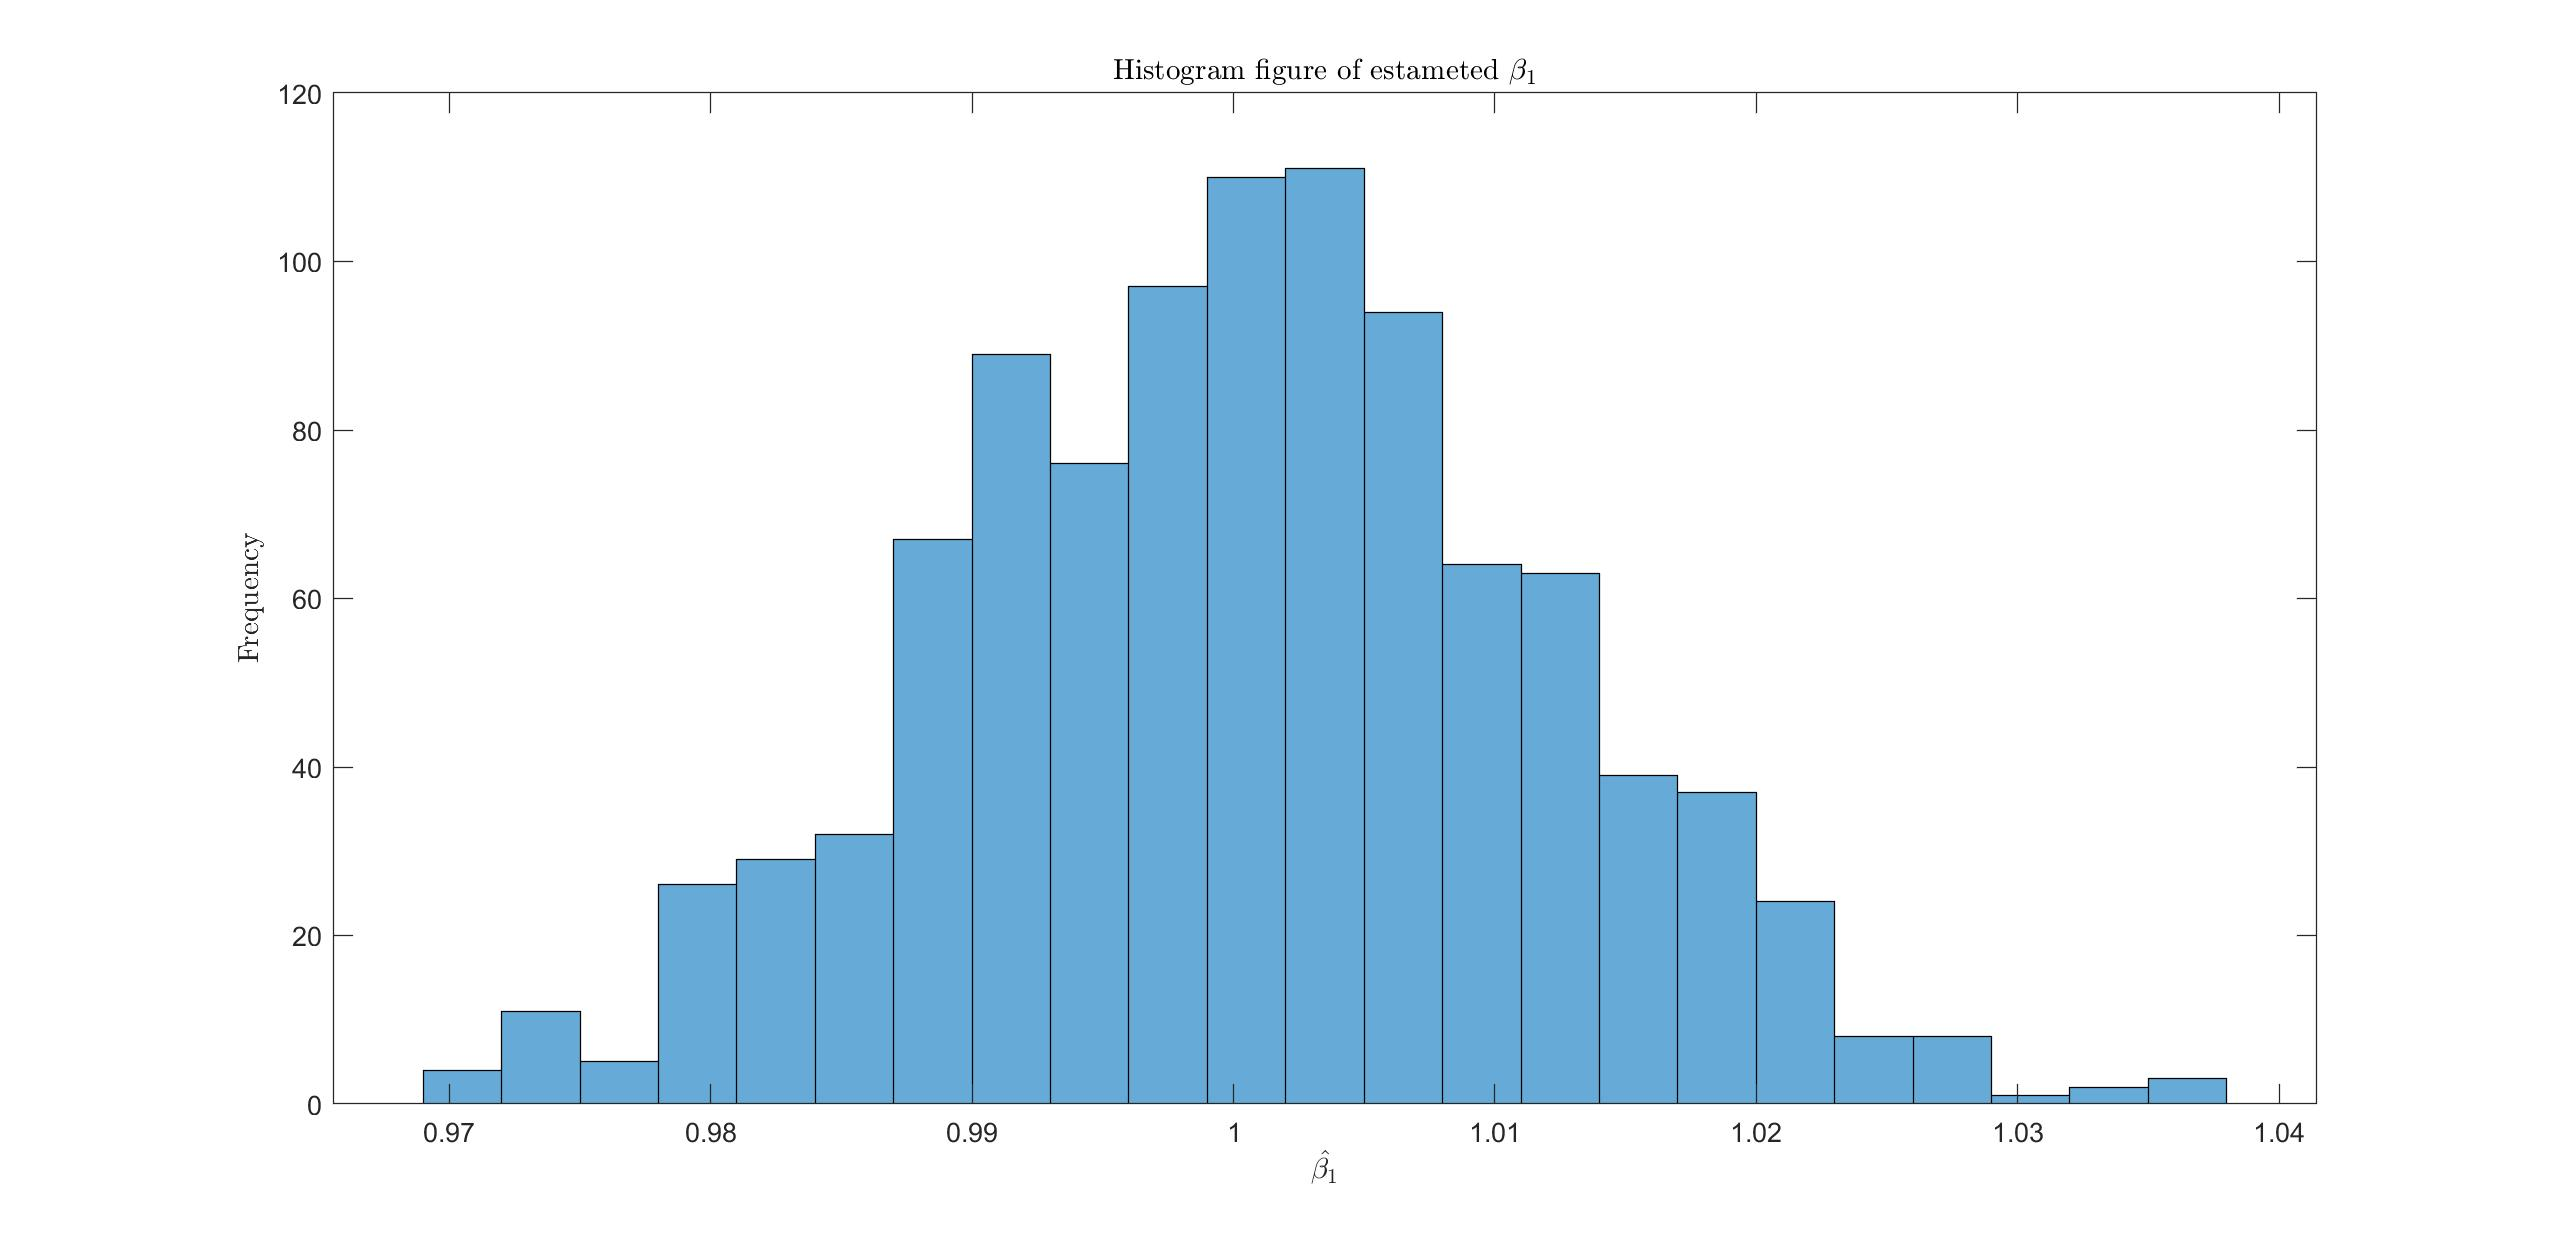
\includegraphics[width=3in]{figures/2Fh1.jpg}
			\end{minipage}
		}
		\centering
		\caption{ Histogram of $\hat{\beta_0}^{*}$ and $\hat{\beta_1}^{*}$}
	\end{figure}
	
	%---2FD---
	
\item	Here are the figures of estimated probability density function of $\hat{\beta_0}^{*}$ and $\hat{\beta_1}^{*}$.
	\begin{figure}[H]
		\subfigure{
			\begin{minipage}[l]{1\linewidth}
				\centering
				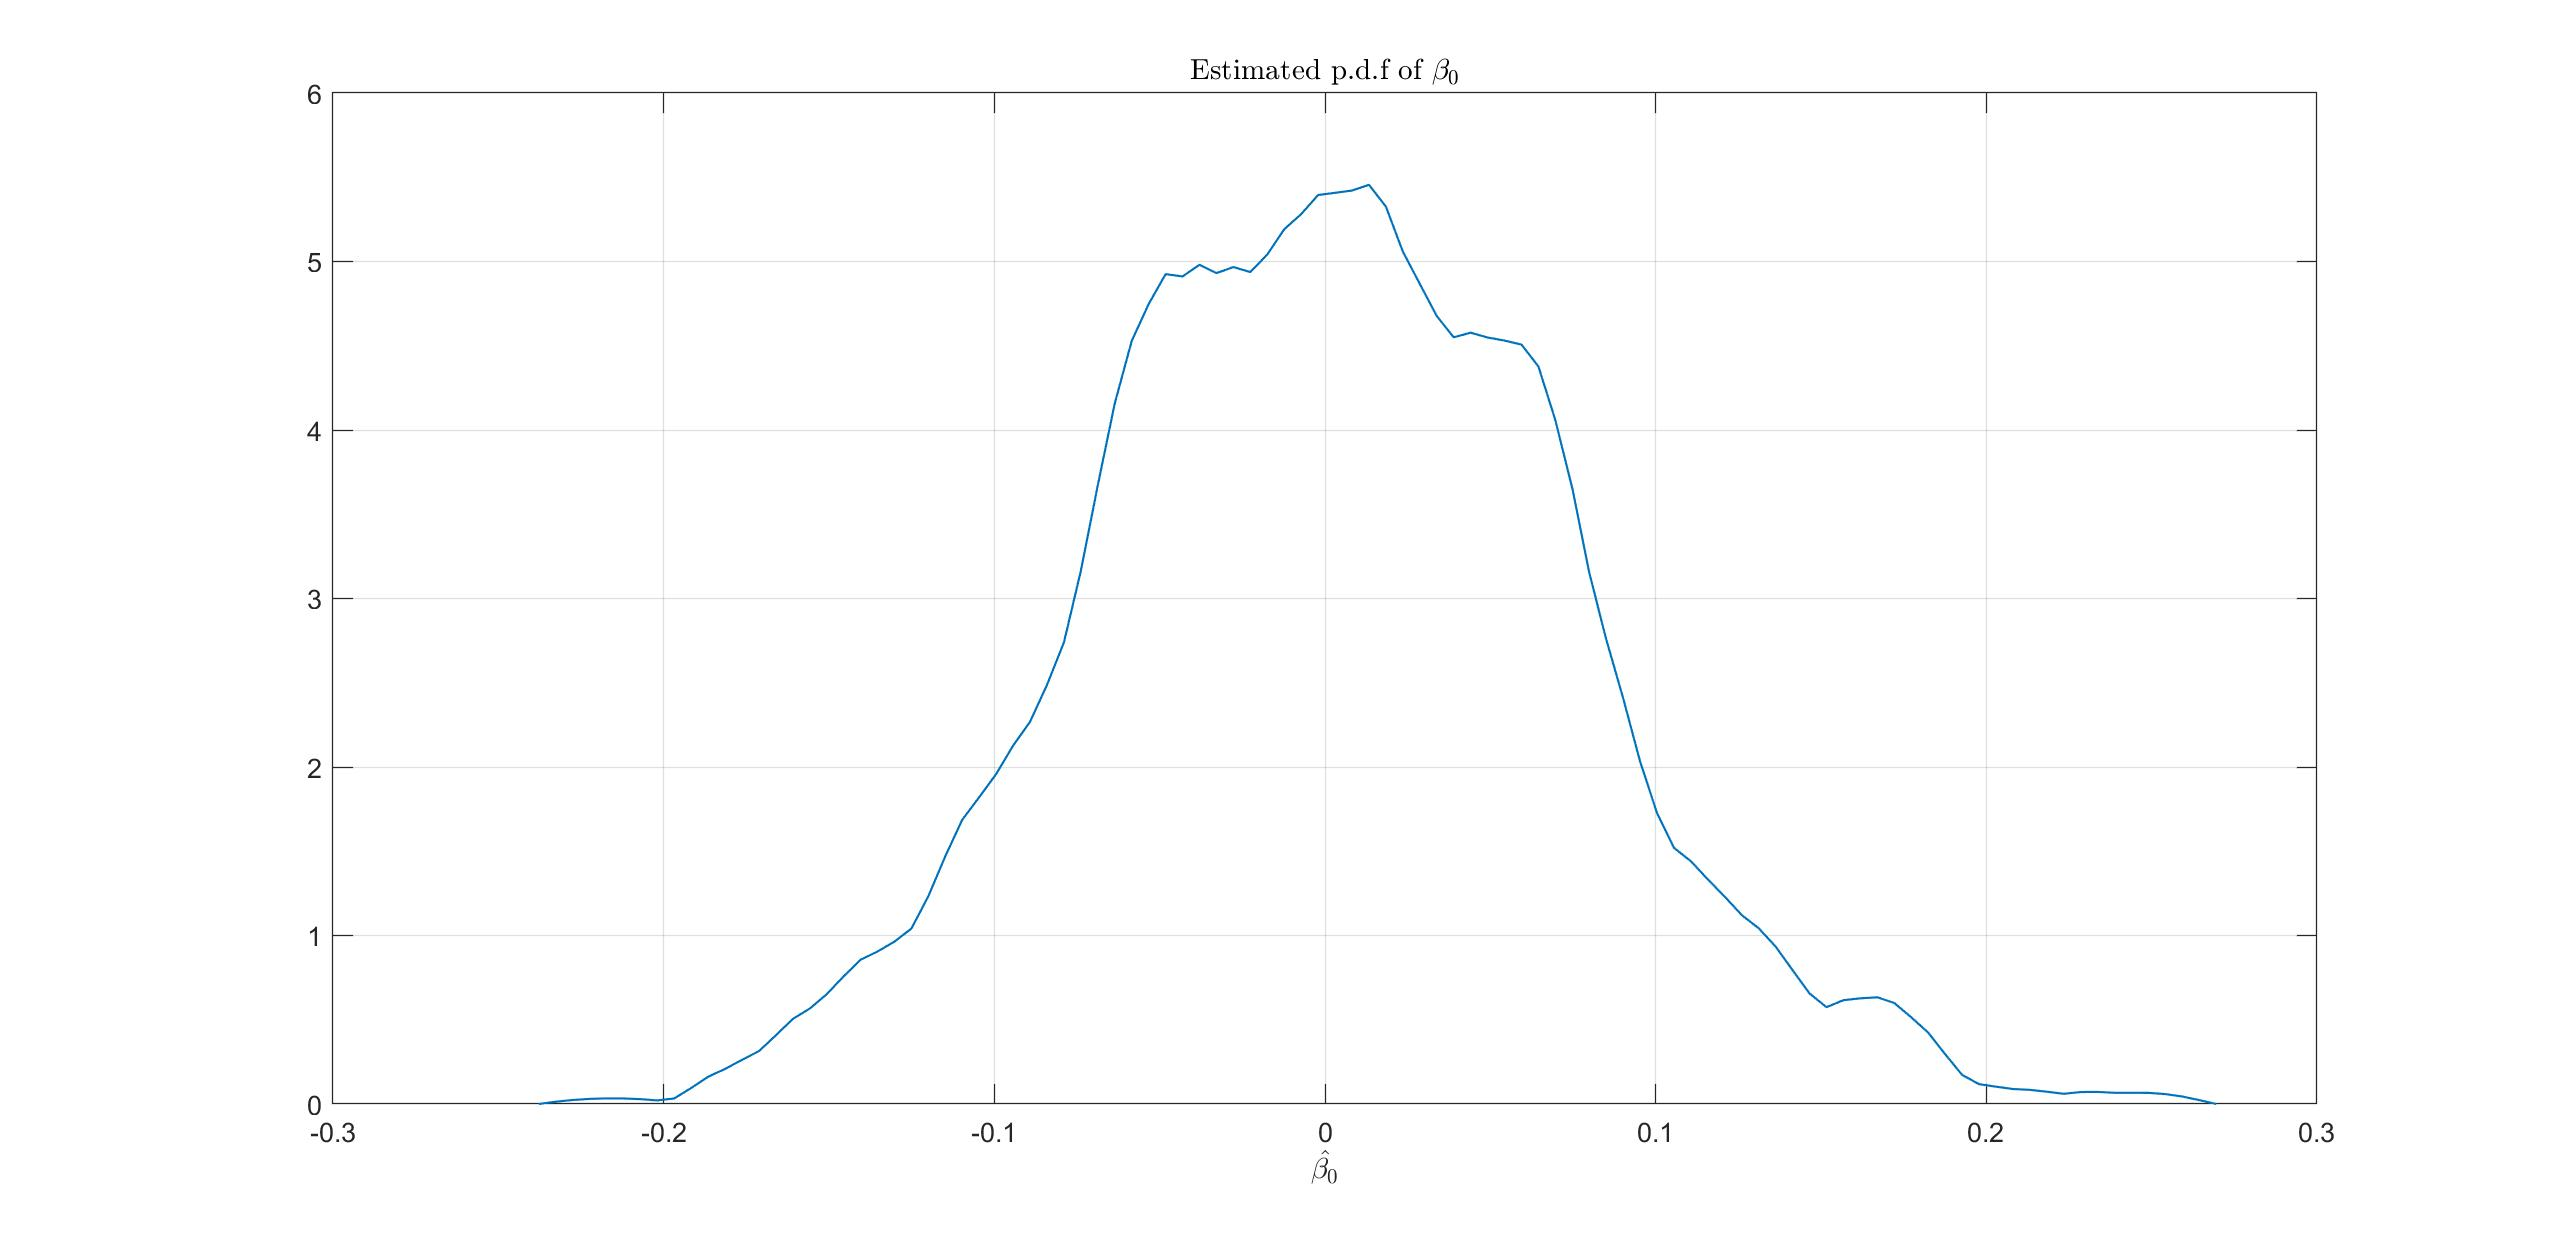
\includegraphics[width=3in]{figures/2Ff0.jpg}
				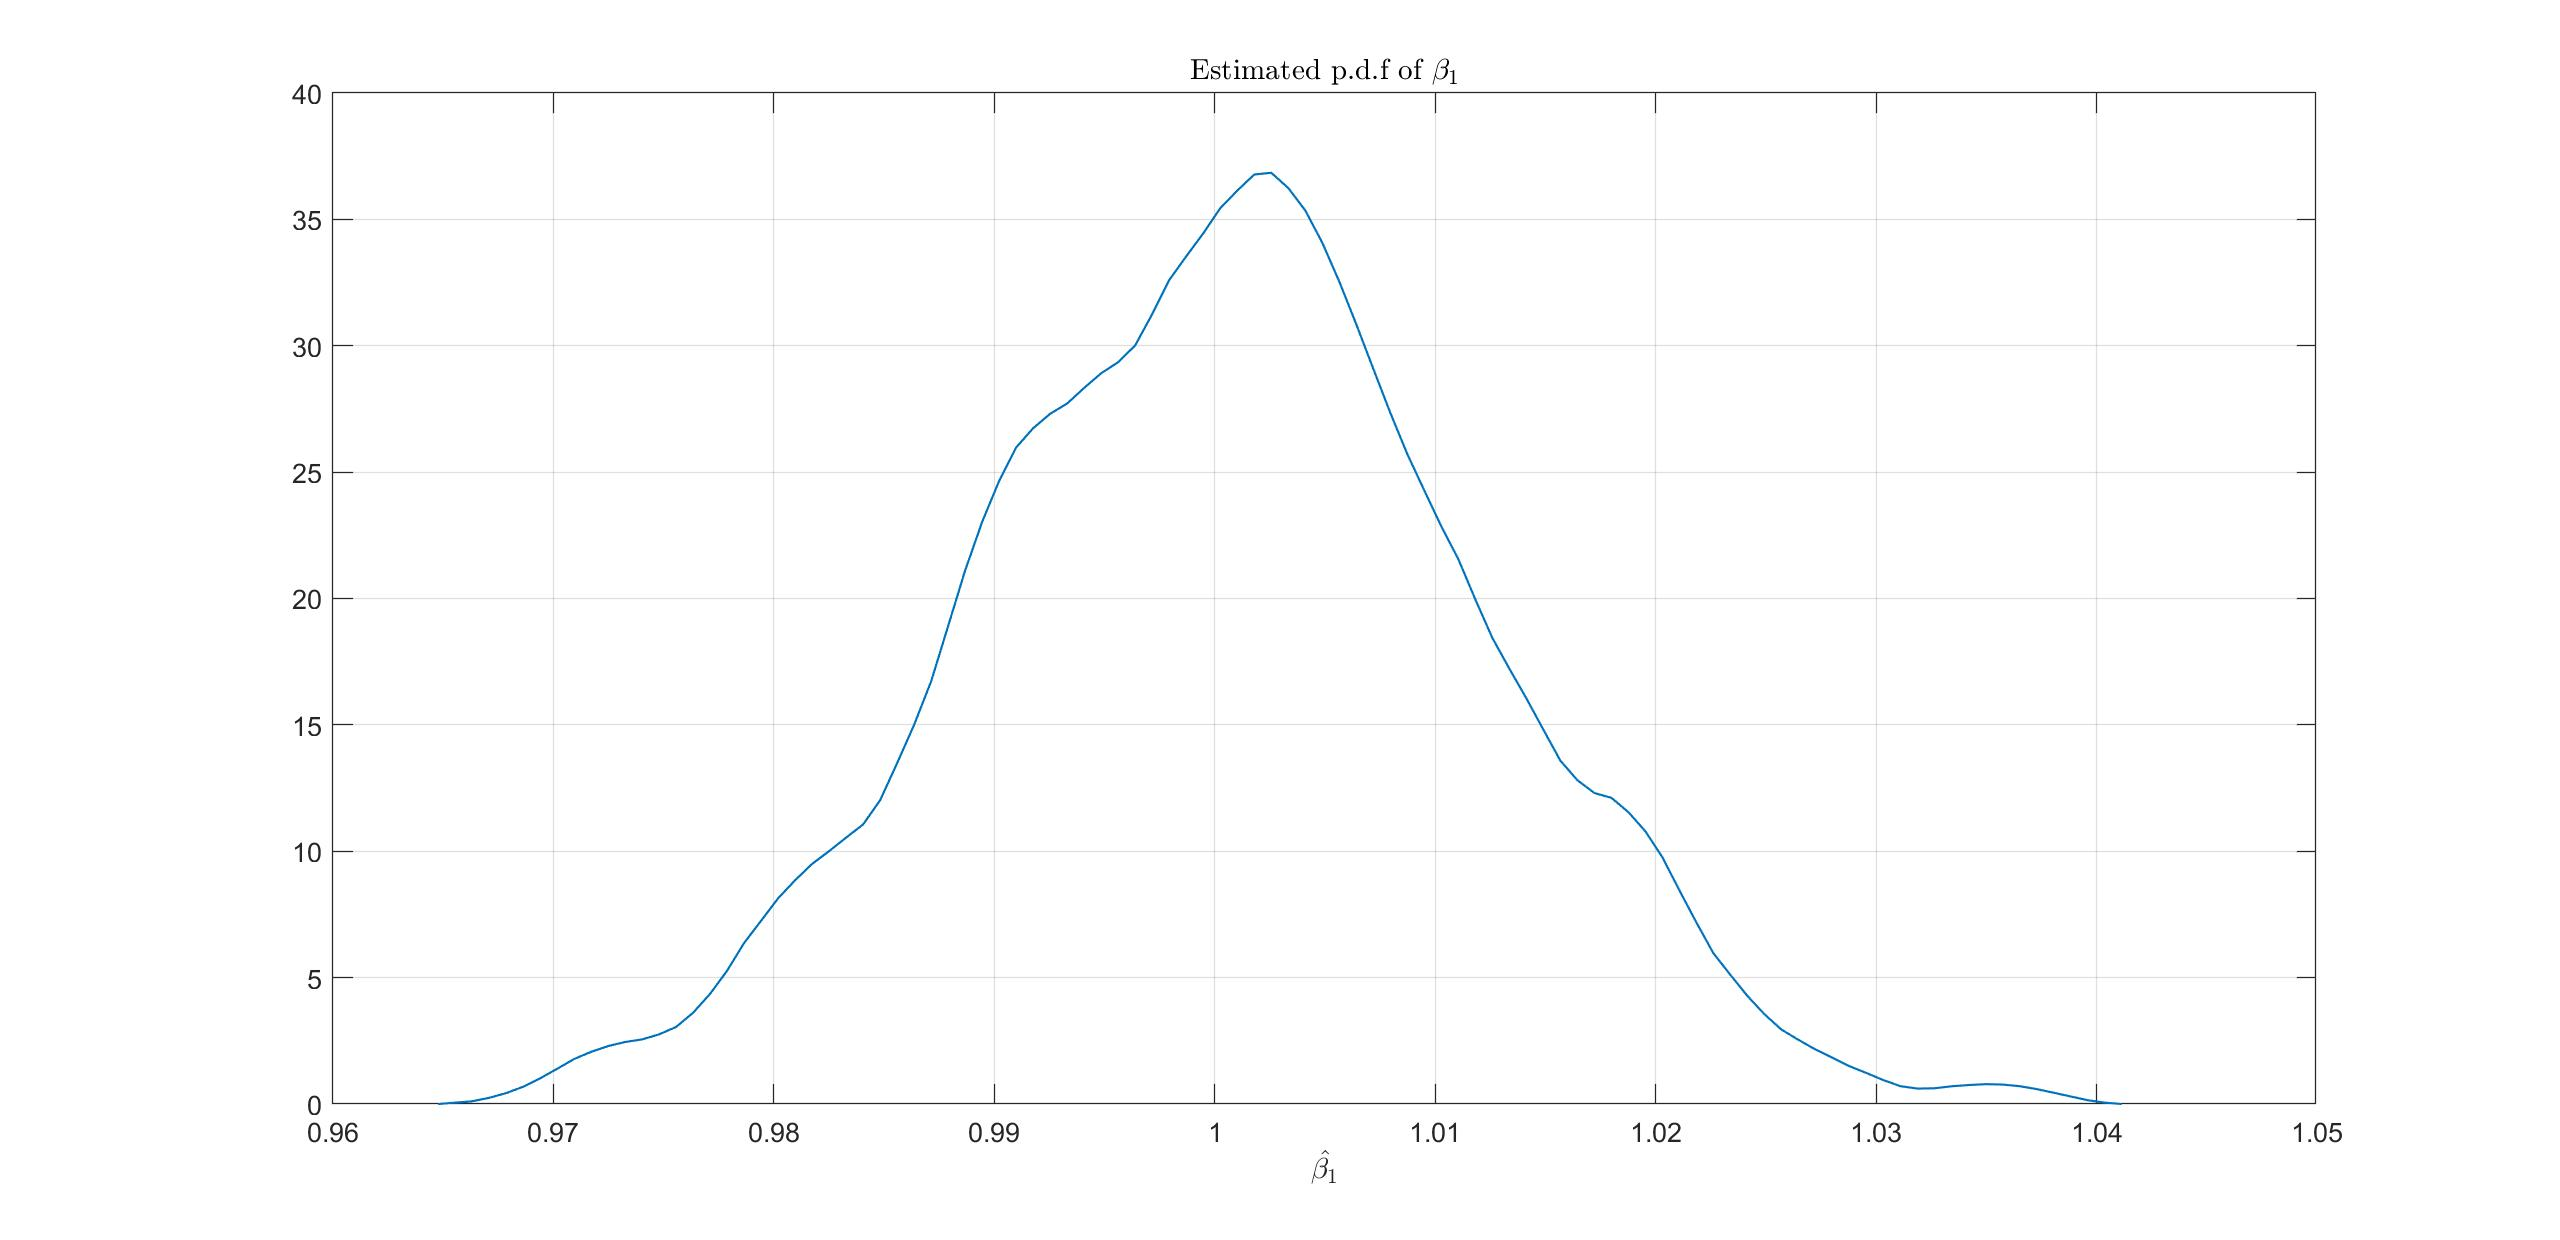
\includegraphics[width=3in]{figures/2Ff1.jpg}
			\end{minipage}
		}
		\centering
		\caption{Histogram of $\hat{\beta_0}^{*}$ and $\hat{\beta_1}^{*}$}
	\end{figure}
\end{enumerate}
From the figures we can see the shape of distribution of $\hat{\beta_0}^{*}$ and $\hat{\beta_1}^{*}$ are little different to normal distribution: they are skewed left and the mean of $\hat{\beta_0}^{*}$ and $\hat{\beta_1}^{*}$ in the estimated distribution are smaller than $\hat{\beta_0}^{*}$ and $\hat{\beta_1}^{*}$ in part E.

If we keep increasing the variance of noises $\eta_i$, the distribution of $\hat{\beta_0}^{*}$ and $\hat{\beta_1}^{*}$ will skew much more to the left , and their mean will deviation more from true value of  $\beta_0$ and $\beta_1$.\\



The \textbf{MATLAB}:

Scripts of Q2
   \lstinputlisting{scripts/ex6_Q2.m}
\end{enumerate}
\newpage




\section*{Exercise 3-Accounting for EIV When Forecasting Variance)}
\begin{enumerate}[label=\textbf{(\Alph*)}]
	%---A---
\item Here is the summary table of MSE of different forecasting model.
\vspace{-5mm}
	\begin{table}[ht]
	\footnotesize
	\caption{Summary Table of AR1,HAR1 and Non-change Model Forecasting}
	\vspace{1mm}
	\centering % used for centering table
	\begin{tabular}{cccccc} % centered columns (4 columns)
		
	%	\hline %inserts double horizontal lines
		% inserts table	%heading
		\hline % inserts single horizontal line
	Stock&$MSE_{AR1}$& $MSE_{HAR1}$&$MSE_{QAR1}$& $MSE_{QHAR1}$& $MSE_{NC}$\\ \hline
	PG&$1.2432* 10^{-8}$&$1.1566* 10^{-8}$&$1.0158* 10^{-8}$&$1.0085* 10^{-8}$&$1.6612*10^{-8}$\\
	DIS&$1.1391* 10^{-8}$&$9.8089* 10^{-9}$&$1.0507* 10^{-8}$&$1.0924* 10^{-8}$&$1.2085* 10^{-8}$\\
	
		\hline %inserts single line		
	\end{tabular}
\end{table} 
\vspace{-5mm}
\item 
According to the MSE table, the model with smallest MSE for PG and DIS is HARQ1 and HAR1 model, respectively. Even though there is no consistently better model for both stock.

%c
\item Here is the summary table of MSE of different forecasting model.
\vspace{-4mm}	
\begin{table}[ht]
	\caption{Forecasting MSE of Different Models $(\times10^{-8} )$}
		\vspace{1mm}
	\centering %
	\footnotesize
		\resizebox{0.8\textwidth}{!}{%
	\begin{tabular}{lccccc}
			\hline 
		\vspace{0.3mm}
		
		\textbf{Stock} & \textbf{AR1} & \textbf{HAR1} & \textbf{ARQ1} & \textbf{HARQ1} & \textbf{NC} \\ 
		
		\hline
		\textbf{AAPL}  & 3.2714       & 2.9762        & 2.7786       & 2.6902         & 3.9421      \\
		\textbf{AXP}   & 3.5744       & 1.5778        & 1.7709       & 1.4288         & 1.8856      \\
		\textbf{BA}    & 2.3167       & 2.1559        & 2.2445       & 2.1558         & 3.3353      \\
		\textbf{BAC}   & 12.7604      & 11.4649       & 12.1244      & 11.0409        & 13.0808     \\
		\textbf{BLK}   & 2.2313       & 1.7329        & 1.7581       & 1.6140         & 2.0247      \\
		\textbf{C}     & 12.1826      & 6.3003        & 6.8755       & 7.9979         & 5.7247      \\
		\textbf{CAT}   & 2.0648       & 1.8225        & 1.9354       & 1.8075         & 2.3188      \\
		\textbf{CSCO}  & 1.0665       & 0.9177        & 0.9491       & 0.8949         & 1.1621      \\
		\textbf{CVX}   & 1.3623       & 1.2868        & 1.3603       & 1.2812         & 1.4211      \\
		\textbf{DIS}   & 1.1391       & 0.9809        & 1.0507       & 1.0924         & 1.2085      \\
		\textbf{GE}    & 3.8628       & 3.3507        & 2.4765       & 2.4125         & 3.8388      \\
		\textbf{GNTX}  & 12.9547      & 11.1596       & 11.9238      & 10.9278        & 18.1811     \\
		\textbf{GS}    & 3.3944       & 2.1976        & 3.1675       & 3.5596         & 2.6432      \\
		\textbf{HD}    & 3.1479       & 2.6523        & 2.3320       & 2.2735         & 3.6952      \\
		\textbf{IBM}   & 0.6825       & 0.6393        & 0.5895       & 0.5903         & 0.7714      \\
		\textbf{INTC}  & 1.8806       & 1.6442        & 1.5698       & 1.5234         & 2.2521      \\
		\textbf{JNJ}   & 7.7365       & 8.0818        & 7.9765       & 8.1612         & 8.7594      \\
		\textbf{JPM}   & 3.4805       & 2.3850        & 2.5029       & 2.4623         & 3.0487      \\
		\textbf{KO}    & 0.3230       & 0.3134        & 0.2769       & 0.2841         & 0.3632      \\
		\textbf{MCD}   & 0.8678       & 0.7321        & 0.6505       & 0.6396         & 0.9998      \\
		\hline
			\end{tabular}}
		\end{table}
	\newpage
	\begin{table}[ht]
		%\caption{Forecasting MSE of Different Models}
		\centering %
		\footnotesize
		\resizebox{0.8\textwidth}{!}{%
	\begin{tabular}{lccccc}
			\hline
		\textbf{Stock} & \textbf{AR1} & \textbf{HAR1} & \textbf{ARQ1} & \textbf{HARQ1} & \textbf{NC} \\ 
		\hline
		\textbf{MET}   & 4.7331       & 3.4626        & 3.8582       & 3.3952         & 4.7734      \\
		\textbf{MMC}   & 1.0222       & 0.7447        & 0.7473       & 0.6641         & 0.8568      \\
		\textbf{MMM}   & 0.9572       & 0.7548        & 0.6677       & 0.6547         & 0.9877      \\
		\textbf{MRK}   & 1.3333       & 0.8740        & 0.8094       & 0.7869         & 1.0468      \\
		\textbf{MS}    & 15.0342      & 8.9090        & 47.5674      & 44.0217        & 8.9950      \\
		\textbf{MSFT}  & 1.9402       & 1.8601        & 1.6777       & 1.6693         & 2.3991      \\
		\textbf{NKE}   & 3.7374       & 3.6169        & 2.7173       & 2.7401         & 4.4002      \\
		\textbf{PFE}   & 1.2692       & 1.1040        & 1.2880       & 1.1690         & 1.5515      \\
		\textbf{PG}    & 1.2432       & 1.1566        & 1.0158       & 1.0085         & 1.6612      \\
		\textbf{PNC}   & 2.2143       & 1.1236        & 1.3913       & 1.2943         & 1.2884      \\
		\textbf{SPY}   & 0.5440       & 0.5224        & 0.4111       & 0.4313         & 0.5580      \\
		\textbf{STT}   & 26.1304      & 6.0592        & 4.7533       & 3.6078         & 2.3478      \\
		\textbf{TSLA}  & 3.6171       & 2.5752        & 3.4272       & 2.6248         & 3.5462      \\
		\textbf{UNH}   & 9.6769       & 8.7356        & 9.0138       & 8.6044         & 14.6258     \\
		\textbf{UTX}   & 0.7892       & 0.7204        & 0.7679       & 0.7382         & 0.9246      \\
		\textbf{VZ}    & 0.7412       & 0.6082        & 0.6622       & 0.6168         & 0.8915      \\
		\textbf{WMT}   & 1.6148       & 1.5385        & 1.5195       & 1.5042         & 2.5851      \\
		\textbf{XOM}   & 0.9464       & 0.8874        & 0.8611       & 0.8410         & 0.9395      \\
		\hline
	\end{tabular}}
\end{table}

From the MSE table we cannot find a model that is consistently better than other models for all stocks, however, we can find two models : HAR1 and Non-change, which are more stable than the AR1, ARQ1 and HARQ1 model for all stocks.

If QIV is much large for the data, using HARQ and ARQ model to reduce the estimate error in beta will be a bad idea since the large QIV will bring more biases for estimating. 

\begin{figure}[H]	
	\centering
	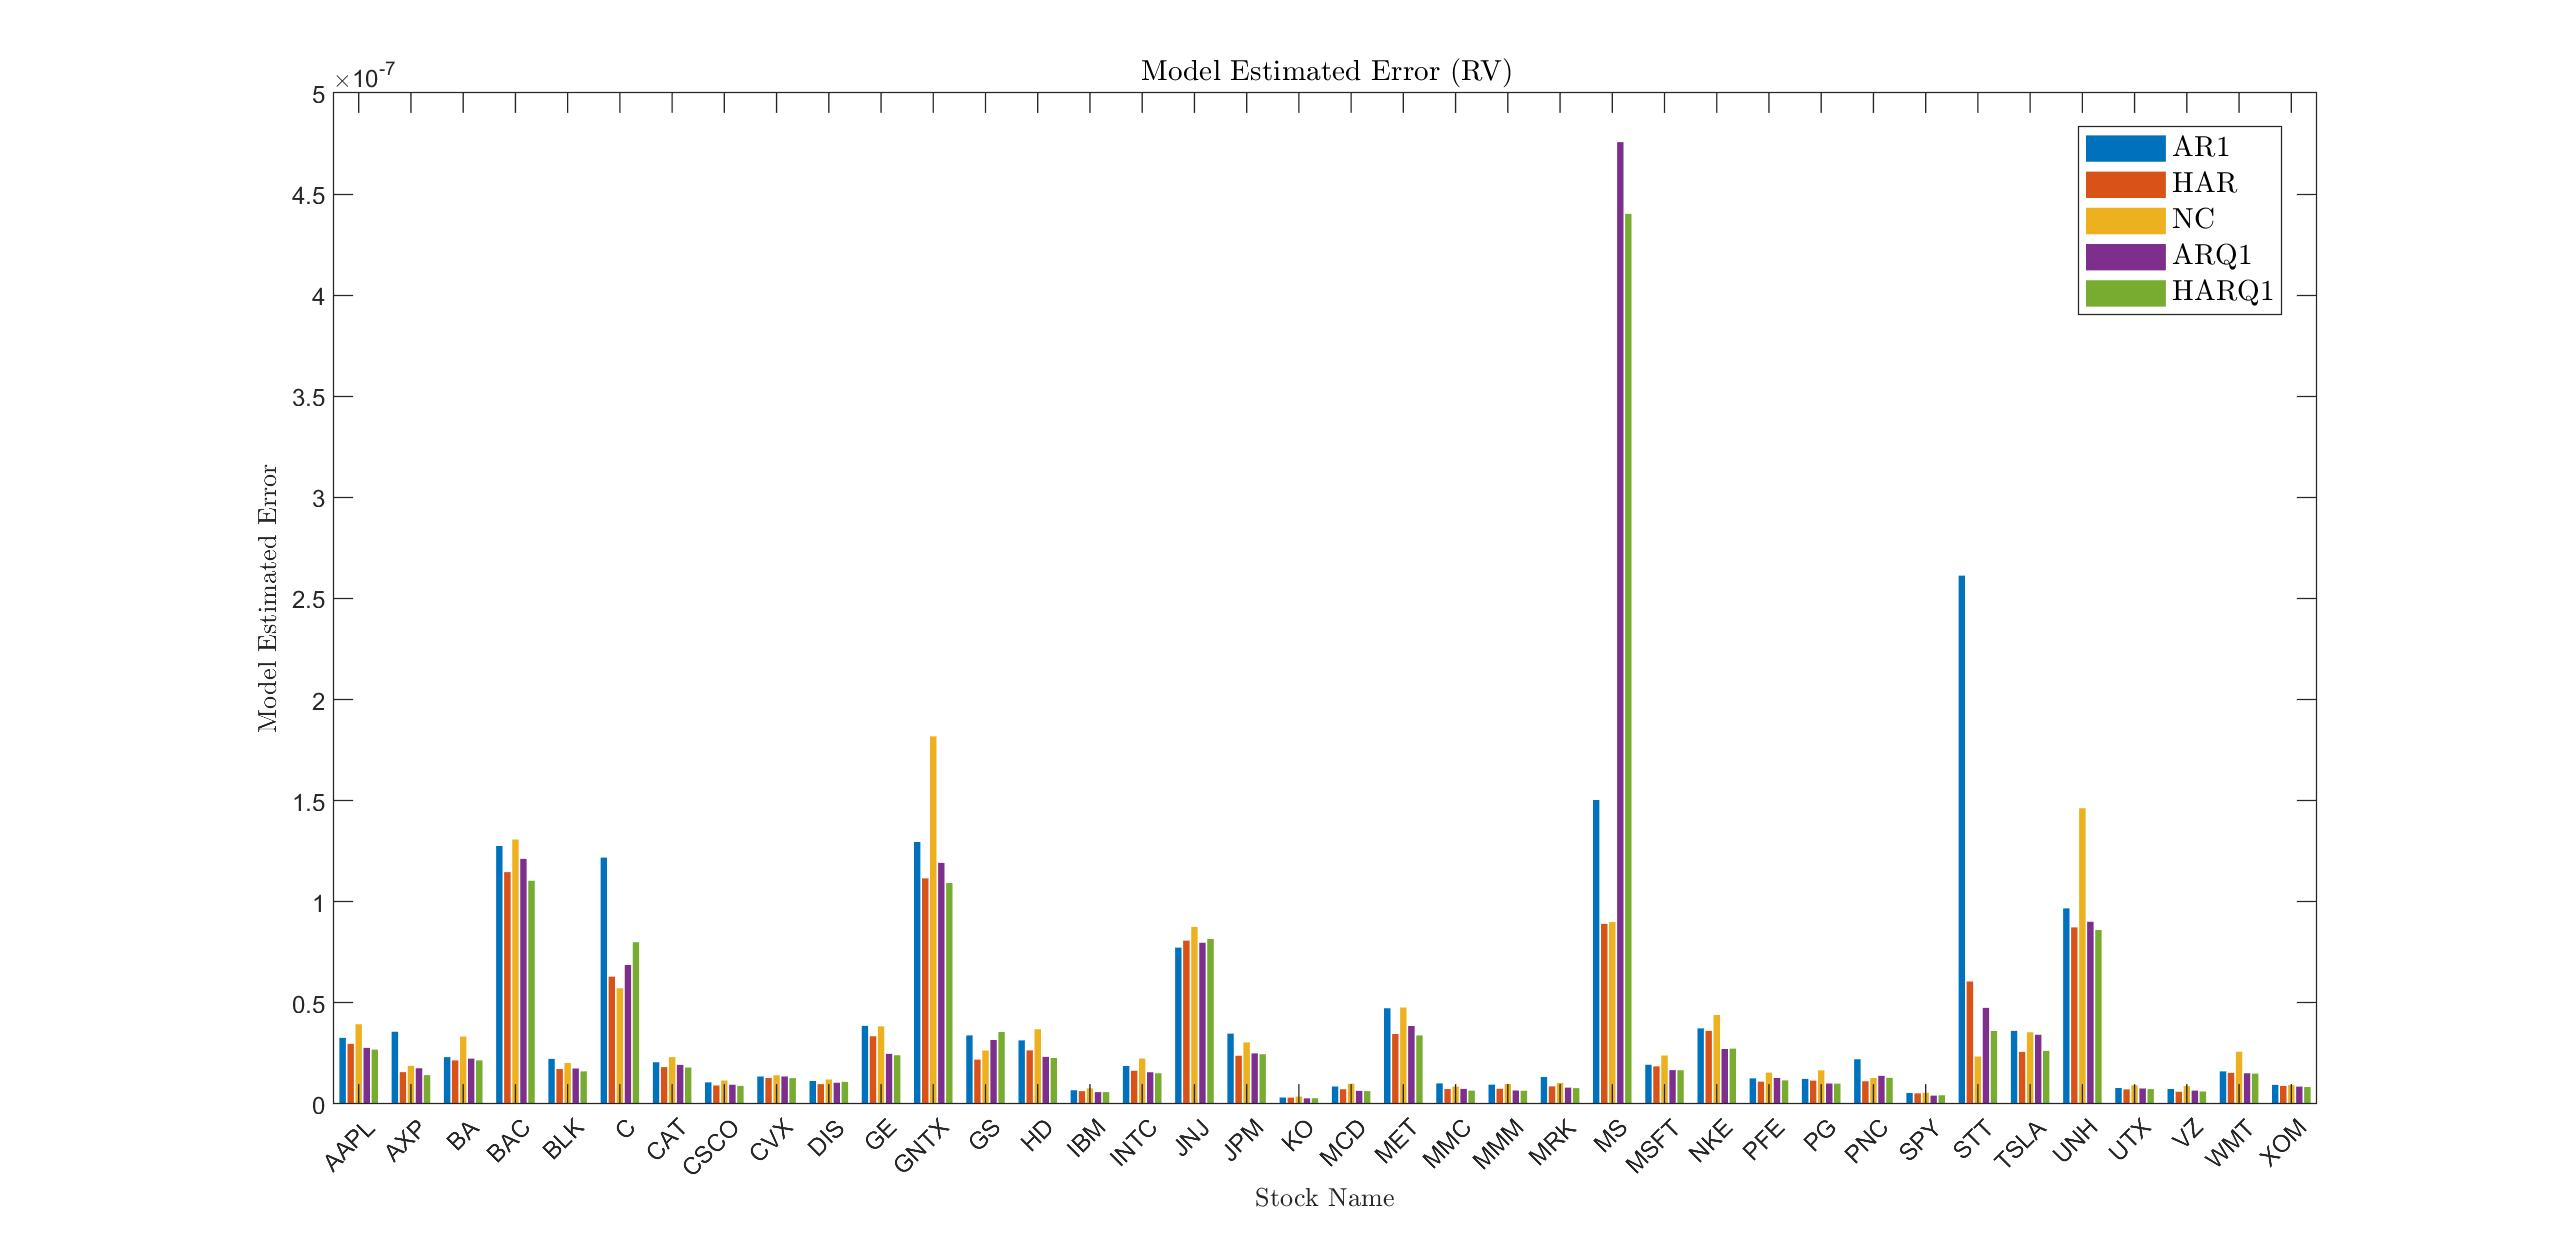
\includegraphics[width=12cm]{figures/3C11.jpg}
	\centering
	\caption{ Bar Plot of RV Forecast MSE}
\end{figure}
\newpage
\begin{figure}[H]	
	\centering
	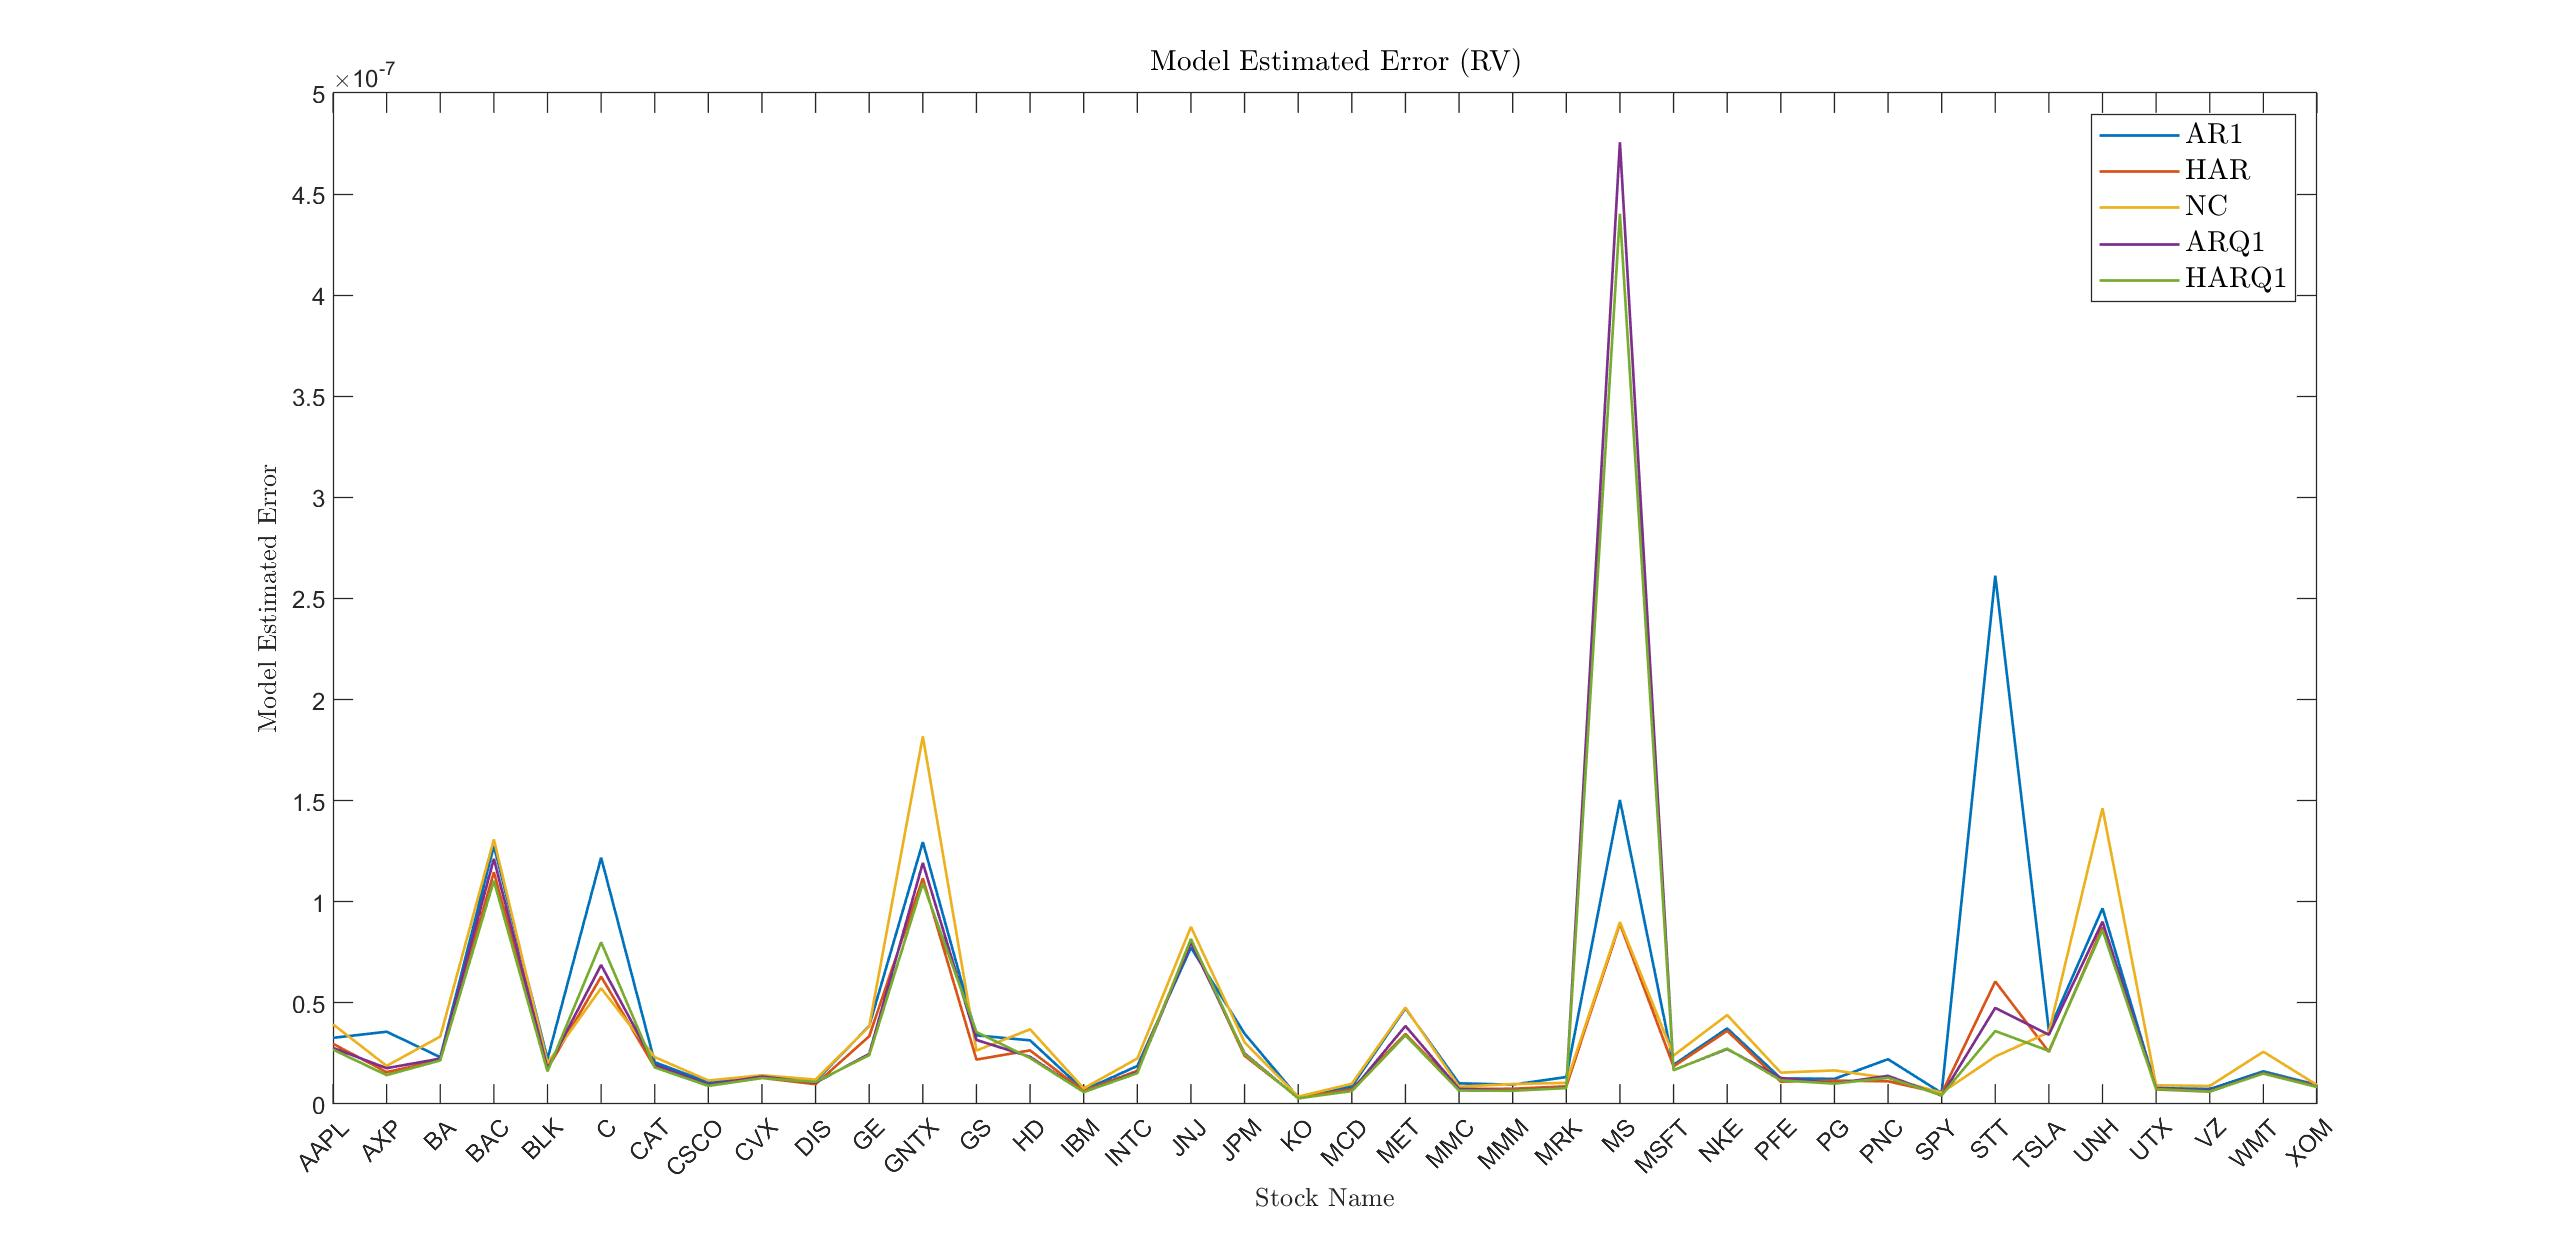
\includegraphics[width=12cm]{figures/3C22.jpg}
	\centering
	\caption{ Figure of RV Forecast MSE}
\end{figure}
From the figures we can clearly find that for most of stocks, the difference of MSE of five models are small, which mean these five models work well in quasi-forecasting. However, for some specific stocks, like MS, QSR1 and QHAR1 work badly and they have about three time MSE as other's. For stock STT, AR1 model works badly and has two times of MSE as others. 

In conclusion, HAR1 and Non-change model are the most stable model and work consistently better for all stocks.


\item   
Here is the summary table of MSE of different forecasting model.
\vspace{-5mm}
\begin{table}[ht]
	\caption{Forecasting MSE of Different Models(TV)$(\times10^{-8} )$}
	\vspace{1mm}
	\centering %
	\footnotesize
	\resizebox{0.8\textwidth}{!}{%	
		\begin{tabular}{lccccc}
			\hline 
			\vspace{0.3mm}
	\textbf{Stock} & \textbf{AR1} & \textbf{HAR1} & \textbf{ARQ} & \textbf{HARQ1} & \textbf{NC} \\	\hline 
	\textbf{AAPL}  & 3.2091       & 2.9623        & 2.7051       & 2.6453         & 3.8653      \\
	\textbf{AXP}   & 3.2987       & 1.4093        & 1.4958       & 1.2628         & 1.5763      \\
	\textbf{BA}    & 2.2521       & 2.0966        & 2.1955       & 2.1188         & 3.1431      \\
	\textbf{BAC}   & 12.5713      & 11.2341       & 12.0602      & 10.9838        & 13.0232     \\
	\textbf{BLK}   & 2.1816       & 1.7107        & 1.7118       & 1.5942         & 1.9908      \\
	\textbf{C}     & 12.6278      & 6.3383        & 6.5516       & 6.7494         & 5.6320      \\
	\textbf{CAT}   & 1.9681       & 1.7371        & 1.8305       & 1.7161         & 2.1880      \\
	\textbf{CSCO}  & 1.0136       & 0.9145        & 1.0763       & 0.9932         & 1.1534      \\ 
	\textbf{CVX}   & 1.3352       & 1.2672        & 1.3759       & 1.2812         & 1.3838      \\
	\textbf{DIS}   & 0.9758       & 0.8681        & 0.8626       & 0.8295         & 1.0034      \\
	\textbf{GE}    & 3.8282       & 3.3438        & 2.4326       & 2.3894         & 3.8257      \\
	\textbf{GNTX}  & 10.1214      & 8.6838        & 8.9482       & 8.3329         & 13.7327     \\
	\textbf{GS}    & 3.1909       & 2.1473        & 3.7833       & 3.8295         & 2.6105      \\ \hline
	
	
		\end{tabular}}
\end{table}
\newpage
\begin{table}[ht]
%\caption{Forecasting MSE of Different Models}
\centering %
\footnotesize
\resizebox{0.8\textwidth}{!}{%
\begin{tabular}{lccccc}
\hline
\textbf{Stock} & \textbf{AR1} & \textbf{HAR1} & \textbf{ARQ} & \textbf{HARQ1} & \textbf{NC} \\ 
\hline
	
	\textbf{HD}    & 3.1849       & 2.7063        & 2.3773       & 2.2965         & 3.6689      \\
	\textbf{IBM}   & 0.6501       & 0.6276        & 0.5924       & 0.5829         & 0.7544      \\
	\textbf{INTC}  & 1.4487       & 1.2924        & 1.2410       & 1.2159         & 1.7189      \\
	\textbf{JNJ}   & 0.2685       & 0.2613        & 0.2680       & 0.2580         & 0.2929      \\
	\textbf{JPM}   & 3.3475       & 2.3436        & 2.4872       & 2.4502         & 2.9863      \\
	\textbf{KO}    & 0.3173       & 0.3107        & 0.2783       & 0.2787         & 0.3566      \\
	\textbf{MCD}   & 0.8562       & 0.7186        & 0.6378       & 0.6286         & 0.9823      \\
	\textbf{MET}   & 4.1713       & 2.9094        & 3.2422       & 2.7849         & 3.7956      \\
	\textbf{MMC}   & 0.8604       & 0.7131        & 0.6189       & 0.6163         & 0.8430      \\
	\textbf{MMM}   & 0.8988       & 0.7535        & 0.7127       & 0.6753         & 0.9757      \\
	\textbf{MRK}   & 1.0049       & 0.7948        & 0.7572       & 0.7199         & 1.0017      \\
	\textbf{MS}    & 14.9350      & 8.3848        & 29.7105      & 29.0690        & 8.8612      \\
	\textbf{MSFT}  & 1.9118       & 1.8309        & 1.6274       & 1.6255         & 2.3419      \\
	\textbf{NKE}   & 3.6420       & 3.5443        & 2.5999       & 2.6164         & 4.2373      \\
	\textbf{PFE}   & 0.8766       & 0.7866        & 0.9020       & 0.8401         & 1.0316      \\
	\textbf{PG}    & 1.2324       & 1.1541        & 0.9917       & 0.9857         & 1.5692      \\
	\textbf{PNC}   & 2.1834       & 1.0978        & 1.3494       & 1.2580         & 1.2398      \\
	\textbf{SPY}   & 0.5394       & 0.5299        & 0.4119       & 0.4260         & 0.5483      \\
	\textbf{STT}   & 25.2062      & 5.9830        & 4.1699       & 3.3472         & 2.1732      \\
	\textbf{TSLA}  & 3.3020       & 2.3677        & 3.1266       & 2.4557         & 3.2622      \\
	\textbf{UNH}   & 9.4701       & 8.5657        & 8.7695       & 8.4156         & 14.3376     \\
	\textbf{UTX}   & 0.7187       & 0.6631        & 0.7325       & 0.6962         & 0.8210      \\
	\textbf{VZ}    & 0.7014       & 0.5765        & 0.6413       & 0.6027         & 0.8256      \\
	\textbf{WMT}   & 1.5999       & 1.5231        & 1.4871       & 1.4766         & 2.5414      \\
	\textbf{XOM}   & 0.9264       & 0.9125        & 0.8453       & 0.8185         & 0.9100      \\  \hline
	\end{tabular}}
\end{table}

From the TV MSE table we can find, the range of TV forecast MSE is $(0.2929\times 10^{-8},2.9711\times 10^{-7})$, which is just a half of the range of RV MSE. Since TV just consider the diffusive return of stocks' log return, this will reduce the effects of jump returns and increase the accuracy of forecast.

\newpage

\begin{figure}[H]	
	\centering
	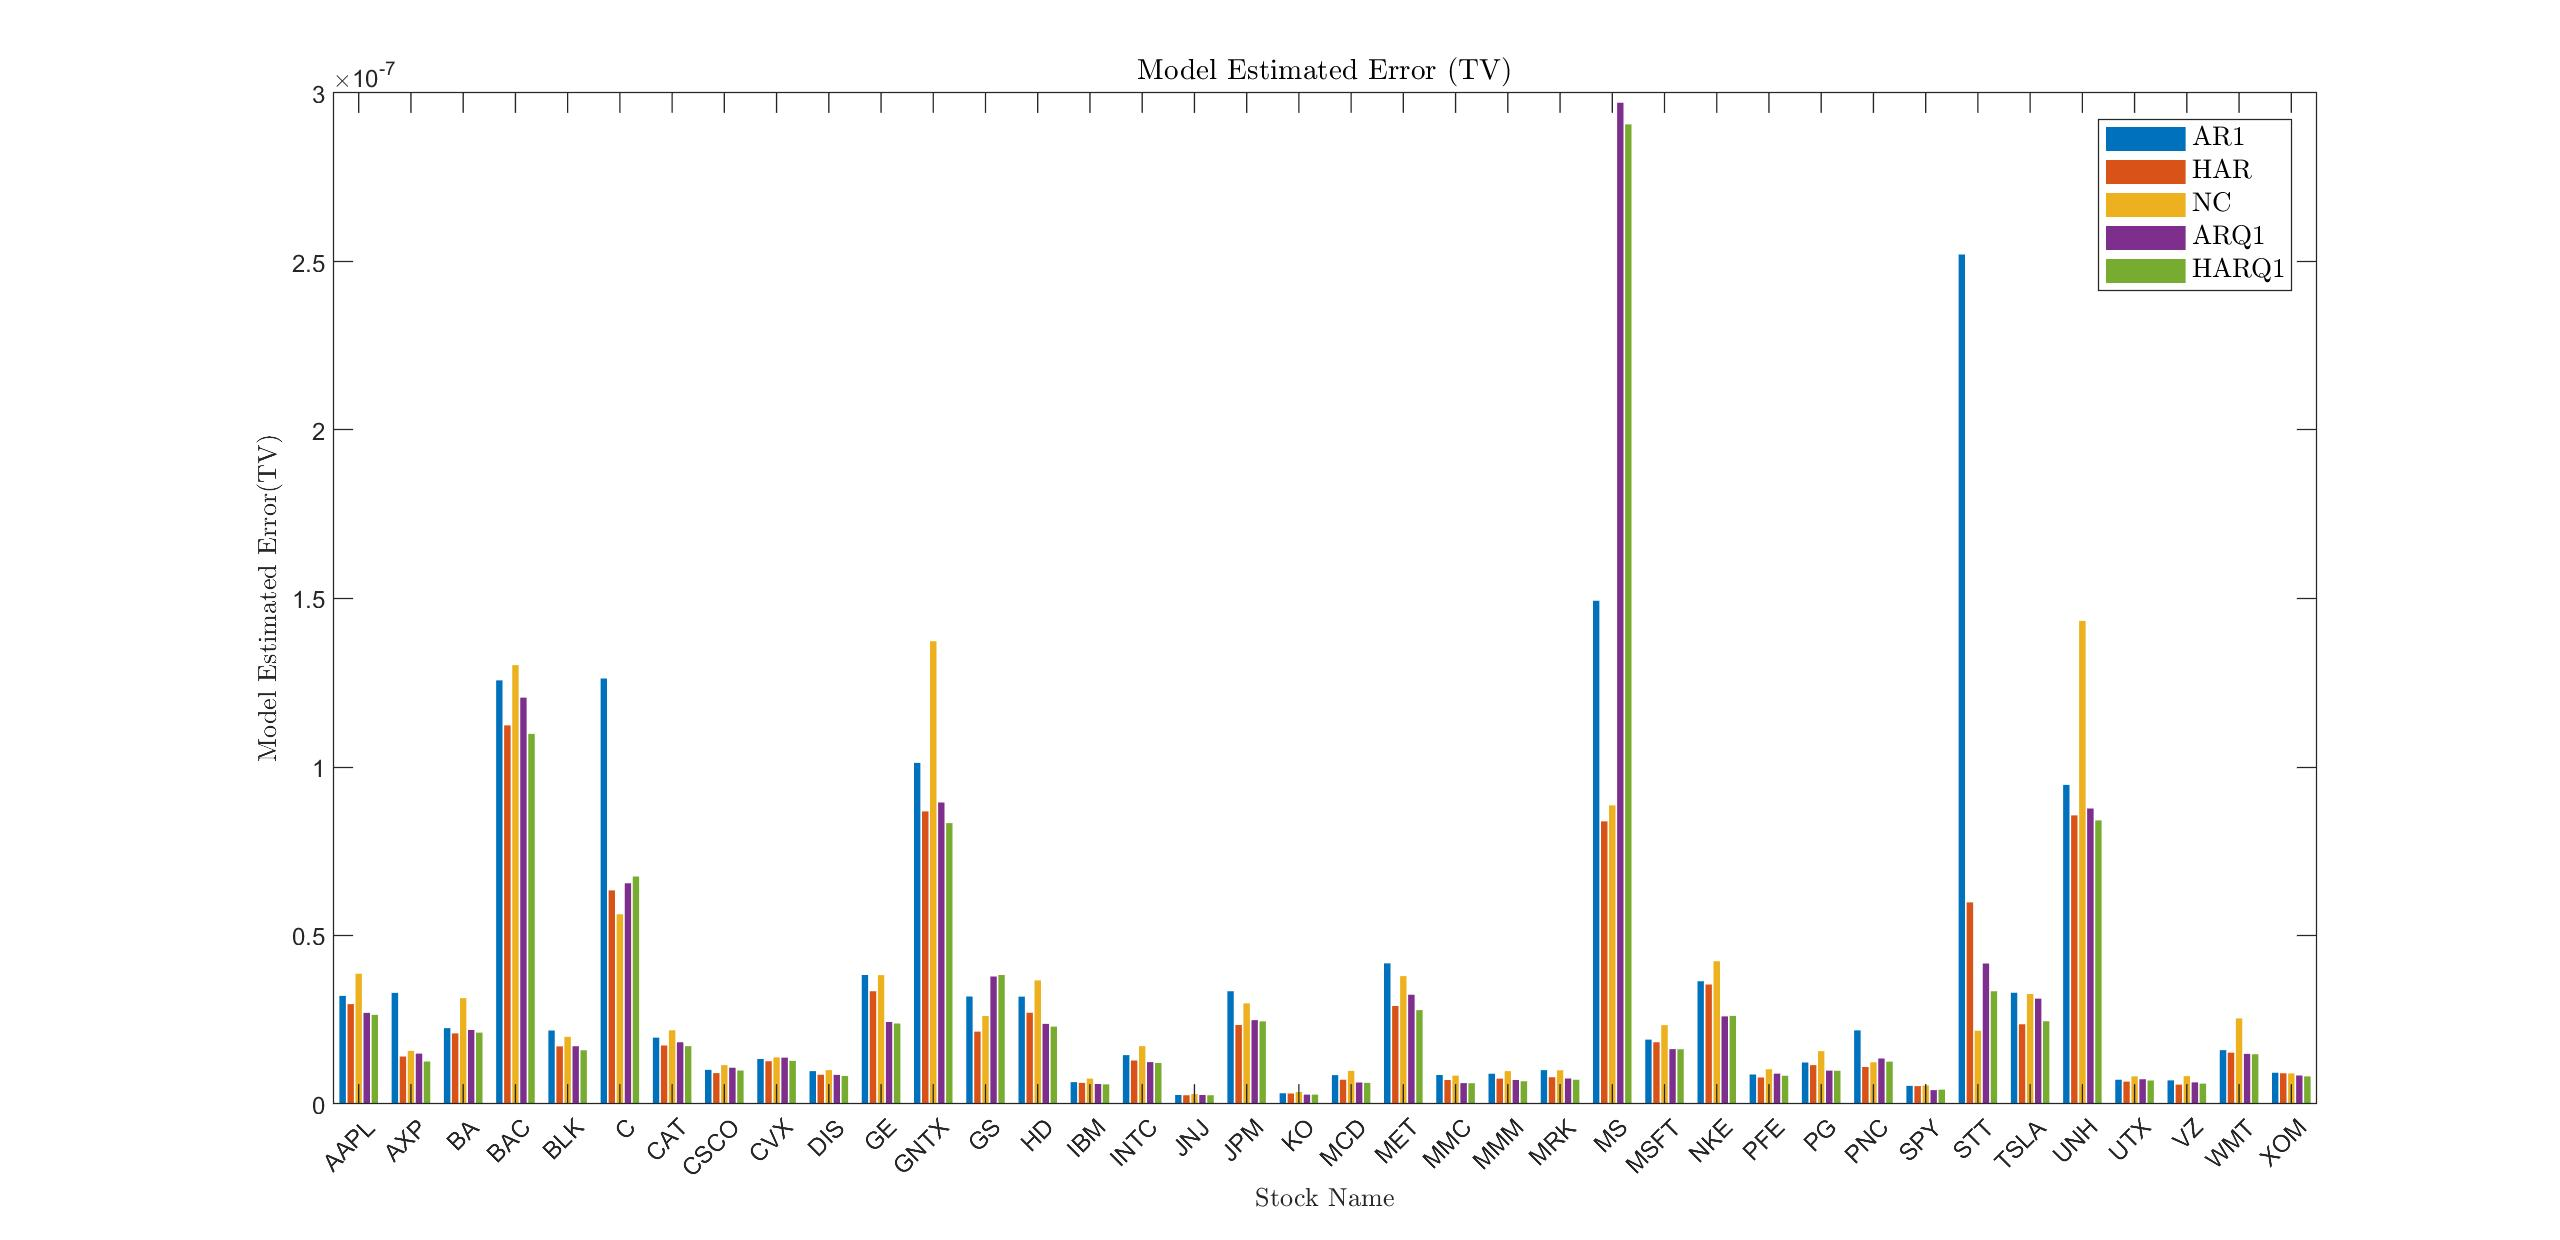
\includegraphics[width=12cm]{figures/3D11.jpg}
	\centering
	\caption{ Bar Plot of TV Forecast MSE}
\end{figure}

\begin{figure}[H]	
	\centering
	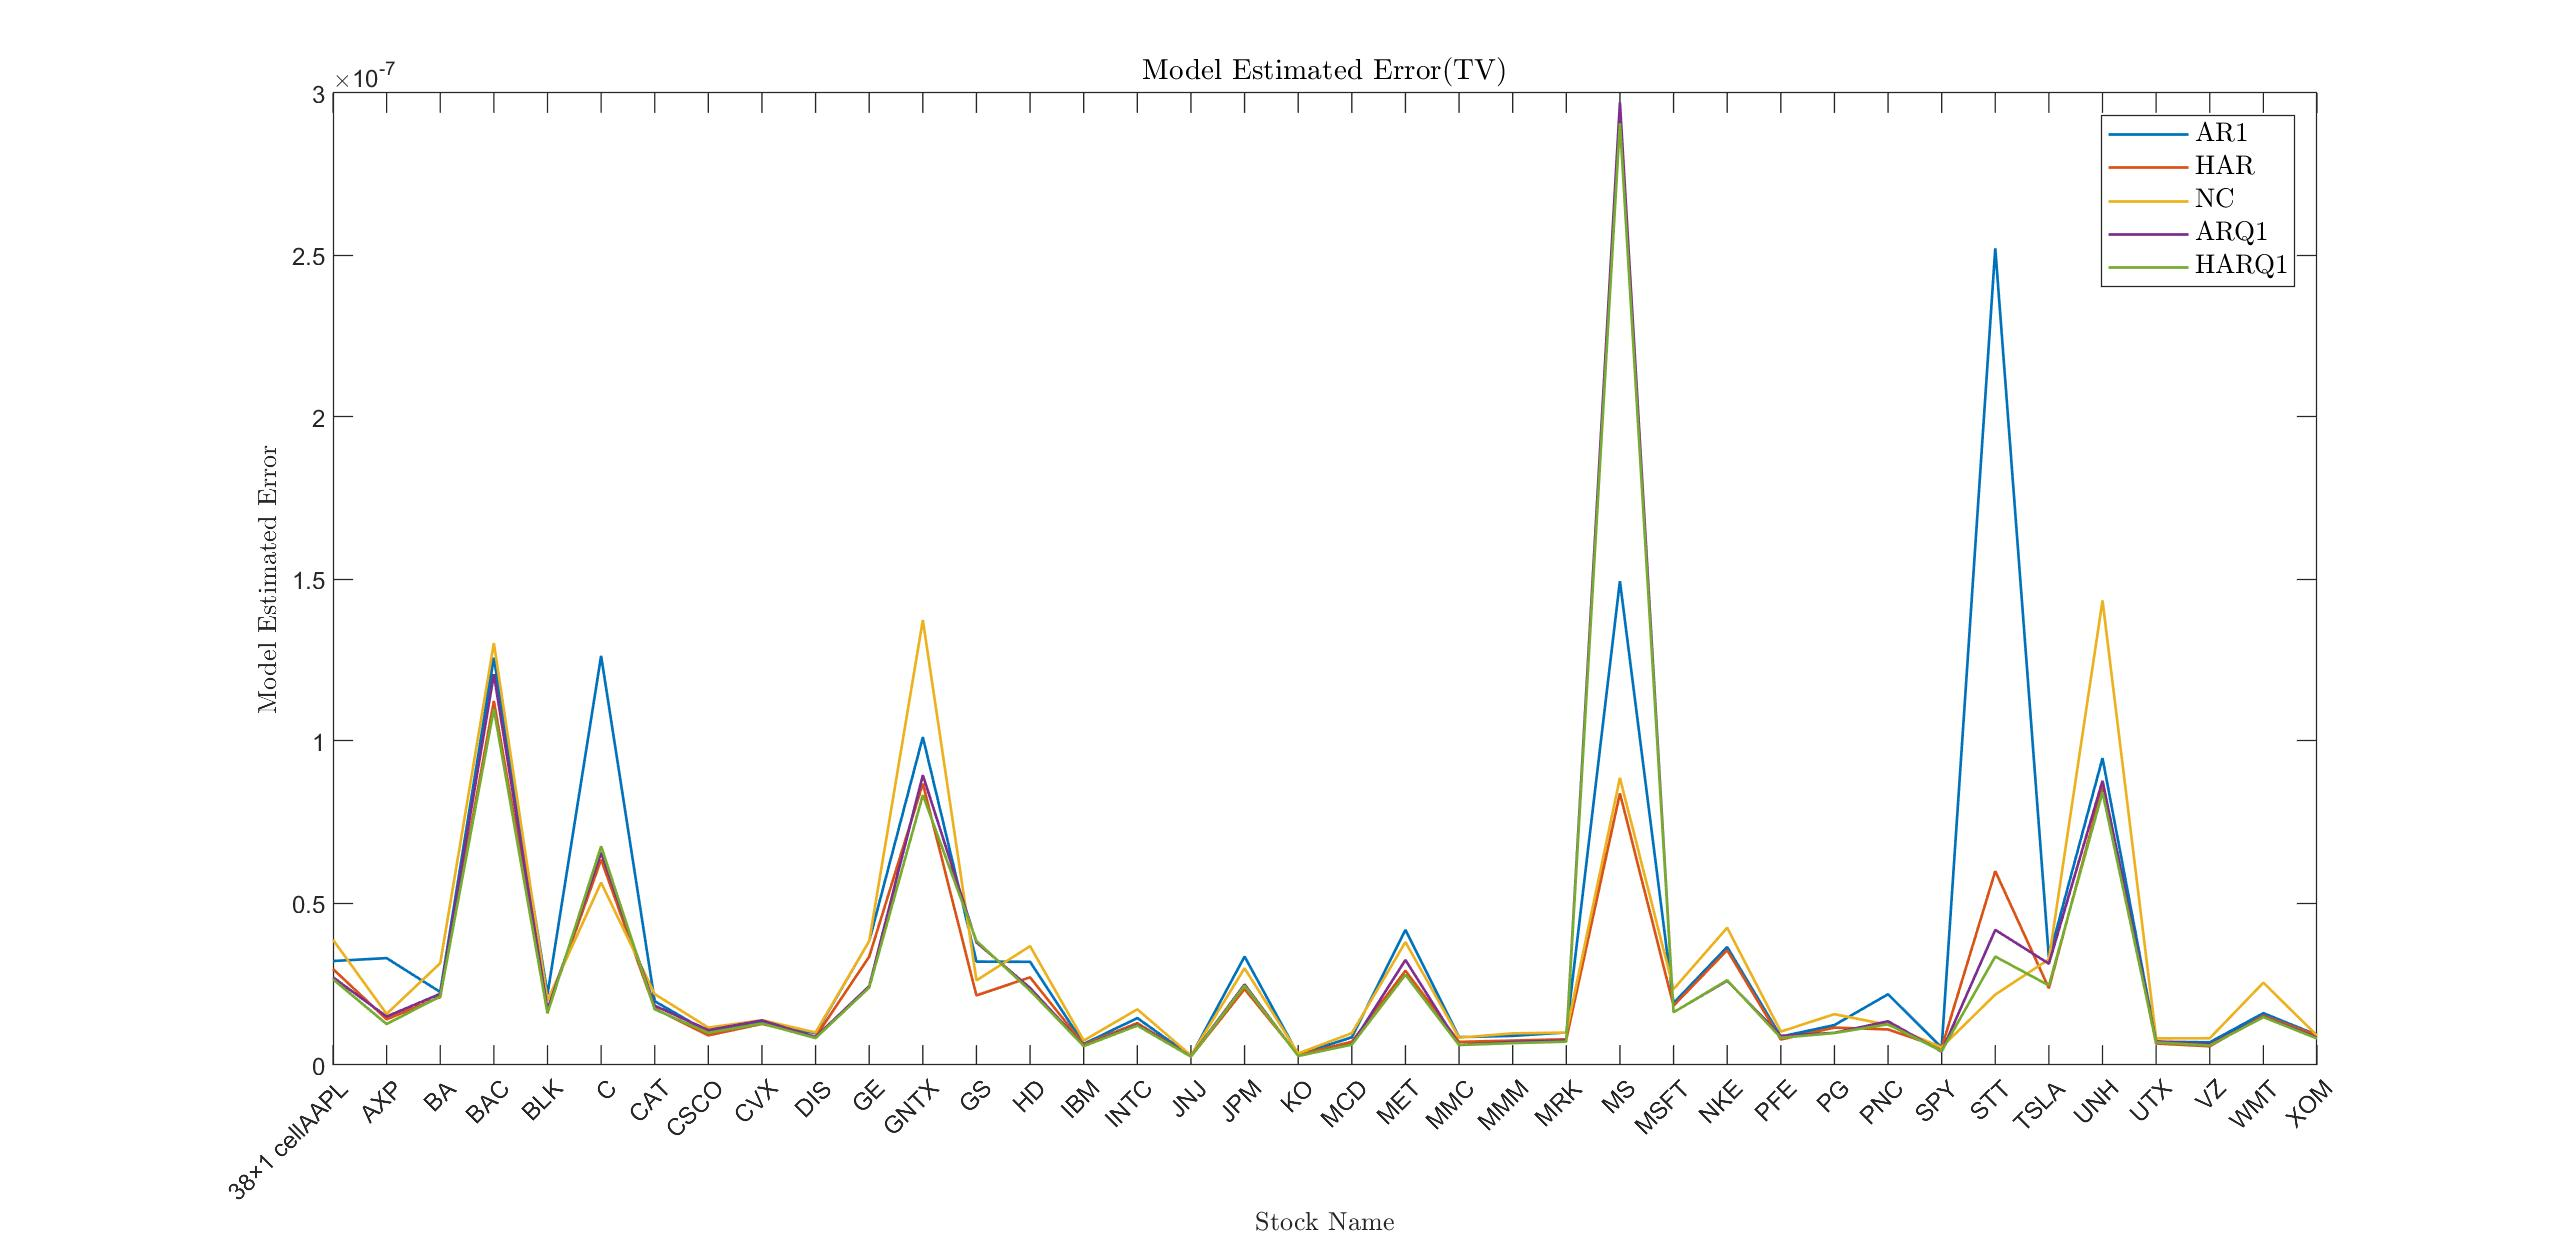
\includegraphics[width=12cm]{figures/3D22.jpg}
	\centering
	\caption{ Figure of TV Forecast MSE}
\end{figure}

From the figures we can find that for most of stocks, these five models all work well and the difference between different models' MSE is very small. However, the same as the case in forecasting RV, there are stocks that some kind of models works badly. For example, HARQ and ARQ have large MSE for stock MS and AR1 model has the largest MSE for stock STT. 

In conclusion, the MSE is smaller when forecasts RV and HAR1 and Non-change model are the most stable model and work consistently better for all stocks.\\

\newpage

%\vspace{-6mm}
The \textbf{MATLAB}:
Scripts of Q3 A-B
\lstinputlisting{scripts/ex6_Q3A_PG.m}
Scripts of Q3 C
\lstinputlisting{scripts/ex6_Q3C.m}
Scripts of Q3 D
\lstinputlisting{scripts/ex6_Q3D.m}
\end{enumerate}
\end{document}
